\documentclass[11pt,a4paper]{report}

% ---------- Packages ----------
\usepackage[utf8]{inputenc}
\usepackage[T1]{fontenc}
\usepackage[a4paper,margin=2cm]{geometry}
\usepackage{setspace}
\usepackage{xcolor}
\usepackage{titlesec}
\usepackage{enumitem}
\usepackage[colorlinks=true, linkcolor=DeepBlue, urlcolor=DeepBlue, citecolor=DeepBlue]{hyperref}
\usepackage[breakable,skins]{tcolorbox}
\usepackage{amsmath}
\usepackage{cite}
\usepackage{graphicx}
\usepackage{float}
\usepackage{caption}
\usepackage{tocloft}
\usepackage{chngcntr}
\usepackage{booktabs}
\usepackage{tabularx}

% ---------- Page layout ----------
\setstretch{1.05}
\setlength{\parindent}{0pt}
\setlength{\parskip}{0.35em}

% ---------- Continuous numbering ----------
\counterwithout{figure}{chapter}
\counterwithout{table}{chapter}
\counterwithout{equation}{chapter}

% ---------- Colors ----------
\definecolor{DeepBlue}{RGB}{20,45,90}
\definecolor{LightGray}{RGB}{245,245,245}
\definecolor{DarkGray}{RGB}{80,80,80}

% ---------- Chapter and TOC formatting ----------
\titleformat{\chapter}[display]
  {\normalfont\huge\bfseries\color{DeepBlue}}
  {\chaptertitlename\ \thechapter}
  {0.4em}
  {}
\titlespacing*{\chapter}{0pt}{-8pt}{18pt}

\renewcommand{\cftchappresnum}{Chapter~}
\setlength{\cftchapnumwidth}{7.2em}

\newcommand{\startappendices}{%
    \appendix
    \addtocontents{toc}{\protect\renewcommand{\protect\cftchappresnum}{Appendix~}}
    \addtocontents{toc}{\protect\setlength{\protect\cftchapnumwidth}{8.0em}}
}

% ---------- Custom Box Styles ----------
\newtcolorbox{sectionintro}[1]{
    colback=white,
    colframe=DeepBlue,
    boxrule=1pt,
    breakable,
    arc=2mm,
    outer arc=2mm,
    left=10pt,
    right=10pt,
    top=4pt,
    bottom=8pt,
    fontupper=\color{black},
    title=\textbf{#1},
    coltitle=white,
    colbacktitle=DeepBlue,
    attach boxed title to top left={yshift=-2mm, xshift=5mm},
    boxed title style={sharp corners=south, size=small},
    before skip=2pt,
    after skip=8pt
}

\newtcolorbox{contentbox}{
    colback=LightGray,
    colframe=LightGray!80!DarkGray,
    boxrule=0.5pt,
    breakable,
    arc=1.5mm,
    outer arc=1.5mm,
    left=10pt,
    right=10pt,
    top=8pt,
    bottom=8pt,
    fontupper=\small
}

\newcommand{\boxitemtitle}[1]{
    \vspace{0.5em}
    {\large\textbf{\color{DeepBlue} #1}}\par
    \vspace{0.8em}
}

\begin{document}

% ==========================================
% COVER PAGE
% ==========================================
\begin{titlepage}
    \begin{flushleft}
        {\LARGE \textbf{EINDHOVEN UNIVERSITY OF TECHNOLOGY}} \\
        \vspace{0.2cm}
        {\large Department of Electrical Engineering} \\
        {\small Electronic System}
    \end{flushleft}

    \vspace{3.5cm}

    \begin{flushleft}
        {\huge \textbf{Internship Report \& Research Logbook}} \\
        \vspace{0.5cm}
        {\Large Topic: Indoor Multi-Target Tracking and Occlusion Reasoning Using Ceiling-Mounted LiDAR}
    \end{flushleft}

    \vspace{3.5cm}

    \begin{flushleft}
        \begin{tabular}{ll}
            \textbf{Student:} & Yehao Chen \\
            \textbf{Student Number:} & 2216655 \\
            \textbf{Email:} & \href{mailto:y.chen13@student.tue.nl}{y.chen13@student.tue.nl} \\
            \textbf{Supervisor:} & Prof. dr. ir. Guido Dolmans \\
            \textbf{Period:} & April 15 -- June 15 (9 weeks, incl. 2 weeks holiday) \\
            \textbf{Credits:} & 10 ECTS (Applicable for HBO graduates)
        \end{tabular}
    \end{flushleft}

    \vfill
    \begin{center}
        {\small This document contains the formal research report and the chronological logbook for the internship project.}
    \end{center}
\end{titlepage}

% Front matter uses roman page numbering.
\pagenumbering{roman}

% ==========================================
% LIST OF ABBREVIATIONS
% ==========================================
\chapter*{List of Abbreviations}
\addcontentsline{toc}{chapter}{List of Abbreviations}

\begin{itemize}[leftmargin=3cm, labelsep=1cm]
    \item[\textbf{CFTA}] Coarse-Fine Triangle Algorithm
    \item[\textbf{DBSCAN}] Density-Based Spatial Clustering of Applications with Noise
    \item[\textbf{DL}] Deep Learning
    \item[\textbf{DMD}] Dynamic Mode Decomposition
    \item[\textbf{EKF}] Extended Kalman Filter
    \item[\textbf{EOA}] Explicit Occlusion Adaption
    \item[\textbf{EOT}] Extended Object Tracking
    \item[\textbf{EPoD}] Expected Probability of Detection
    \item[\textbf{FPS}] Frames Per Second
    \item[\textbf{GMM}] Gaussian Mixture Model
    \item[\textbf{ID}] Identification
    \item[\textbf{IMU}] Inertial Measurement Unit
    \item[\textbf{IMM}] Interacting Multiple Model
    \item[\textbf{IoU}] Intersection over Union
    \item[\textbf{KDRQ}] KD-tree Range Query
    \item[\textbf{KF}] Kalman Filter
    \item[\textbf{LiDAR}] Light Detection and Ranging
    \item[\textbf{MC}] Monocular Camera
    \item[\textbf{PCA}] Principal Component Analysis
    \item[\textbf{RIBS}] Range and Intensity Background Subtraction
    \item[\textbf{R-LIOM}] Reflectivity-Aware LiDAR-Inertial Odometry and Mapping
    \item[\textbf{ROI}] Region of Interest
    \item[\textbf{RQ}] Research Question
    \item[\textbf{RTS}] Rauch--Tung--Striebel
    \item[\textbf{ZUPT}] Zero-Velocity Update
\end{itemize}

\newpage
\tableofcontents
\newpage

% Main matter starts from Introduction as page 1.
\pagenumbering{arabic}

% ==========================================
\chapter{Introduction}
% ==========================================

\section*{Background and Motivation}
Based on Yiyun Xu's previous research~\cite{xu2026indoorlocalization}, background subtraction and single-target tracking have been validated in a specific indoor configuration using a ceiling-mounted LiDAR at a height of 2.7~m. However, a major challenge appears when the system is extended from 1 target to multiple targets. When persons move close to each other, tracking performance can degrade because of point-cloud merging, mutual occlusion, and temporary detection loss. Therefore, this 7-week internship project investigates the transition from single-target localization to multi-target tracking. The objective is to develop lightweight LiDAR-intrinsic reasoning methods for handling occlusion and merging ambiguities without relying on external visual cues such as camera fusion.

\section*{Research Questions}
This project is structured around 4 research questions:

\begin{enumerate}[leftmargin=*]
    \item \textbf{RQ1:} Can a ceiling-mounted LiDAR reliably separate and track multiple persons, using Yiyun Xu's single-person tracking framework as the baseline?
    \item \textbf{RQ2:} Can a ceiling-mounted LiDAR reliably separate and track a heterogeneous mix of multiple targets, specifically persons and robots?
    \item \textbf{RQ3:} Under which conditions does the tracking system fail, especially due to occlusion, spatial proximity, and point-density degradation?
    \item \textbf{RQ4:} Is the resulting tracking trajectory quality sufficient to serve as an offline ground-truth evaluation standard?
\end{enumerate}

The theoretical analysis is presented in Chapter~2, and the direct answers to the research questions are summarized in Chapter~3.

\newpage

% ==========================================
\chapter{Core Issues: Occlusion and Merging}
% ==========================================



\boxitemtitle{2.1 Simulation Setup}

\begin{contentbox}
\small
\setlength{\abovedisplayskip}{4pt}
\setlength{\belowdisplayskip}{4pt}
\setlength{\tabcolsep}{4pt}
\renewcommand{\arraystretch}{1.08}

\subsection*{Simulation Framework}

Due to the limited availability of multi-target ceiling-mounted LiDAR datasets, a simulation framework is introduced for preliminary analysis before real multi-person data collection. The goal is not to reproduce every hardware-level detail of the Ouster sensor, but to build a controllable and interpretable model for studying when LiDAR-only tracking starts to fail.

\vspace{0.35em}

The framework contains 3 main modules. 1) The \textbf{point-cloud generation} module produces simplified human targets using a ceiling-mounted OSDome-like LiDAR model. It considers body geometry, a rounded head--shoulder cap, gait oscillation, range noise, distance-dependent sparsity, and visibility-dependent point distribution. 2) The \textbf{clustering and trajectory prediction} module estimates target positions frame by frame from the generated point clouds. This module is independent from the ground-truth trajectory, so the tracker does not directly know the true target center. 3) The \textbf{evaluation} module compares tracking performance based on criteria such as ID loss, merged-frame ratio, and trajectory quality.

\vspace{0.45em}

\begin{center}
\begin{minipage}{0.6\linewidth}
    \centering
    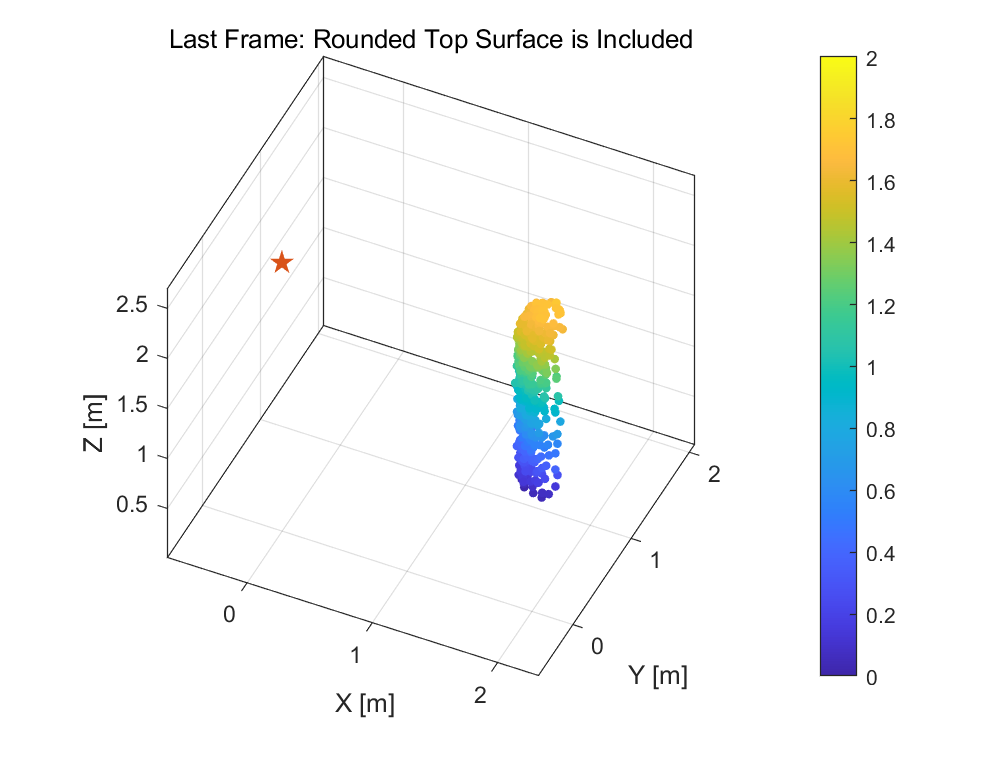
\includegraphics[width=\linewidth]{Figure3.png}

    \vspace{-0.2em}
    \scriptsize (a) Simulated point-cloud distribution in 1 frame.
\end{minipage}
\hfill
\begin{minipage}{0.35\linewidth}
    \centering
    \scriptsize
    \begin{tabularx}{\linewidth}{@{}lX@{}}
    \toprule
    \textbf{Parameter} & \textbf{Value} \\
    \midrule
    LiDAR type & OSDome  \\
    LiDAR height & $2.70~\mathrm{m} (0,0,2.7)$ \\
    Frame rate & $10~\mathrm{Hz}$ \\
    Azimuth samples & $1024$ \\
    Vertical rings & $64$ \\
    Beam angle range & $1^\circ$--$88^\circ$ \\
    Human height & $1.72~\mathrm{m}$ \\
    Body radius & $0.24~\mathrm{m}$ \\
    Cap start height & $1.42~\mathrm{m}$ \\
    Cap vertical height & $0.30~\mathrm{m}$ \\
    Cap shape & rounded upper dome \\
    Range noise & $0.010~\mathrm{m}$ \\
    Distance exponent & $\gamma=1.1$ \\
    Keep strength & $\lambda=0.45$ \\
    Gait amplitude & $0.030~\mathrm{m}$ \\
    Walking speed & $0.55~\mathrm{m/s}$ \\
    \bottomrule
    \end{tabularx}

    \vspace{0.25em}
    \scriptsize (b) Main parameters used in the simulation.
\end{minipage}

\vspace{0.25em}
\captionof{figure}{Single-frame point-cloud generation and main simulation parameters.}
\label{fig:single_frame_and_parameters}
\end{center}

\vspace{0.35em}

Compared with the earlier surface-sampling model, the updated point-cloud generation uses a ray-casting strategy. Each angular cell of the LiDAR emits 1 ray, and each ray contributes at most 1 initial-return point after intersecting with the simplified human model. Therefore, the visible surface and distance-dependent sparsity are produced more naturally by the sensor geometry itself, instead of generating a complete object surface and then manually deleting points. The next part further explains ray-casting and density decay as distance increases.
\newpage

\subsection*{Ray-Casting Model and Density Attenuation}

To seamlessly integrate the aforementioned parameters, the point-cloud generator replicates the physical ray-casting mechanism of an Ouster LiDAR onto a customized dome-cylinder model. For instance, an OS1 model with a $1024 \times 128$ resolution operating at 10 Hz casts approximately 1.31 million rays per frame. While virtual rays propagate indefinitely, this casting mechanism intuitively explains point cloud acquisition: as the rays travel farther, the unit area they cover expands, which inherently reduces the spatial point density.

This density attenuation phenomenon can be interpreted through 2 perspectives:
\begin{itemize}
    \item \textbf{Coordinate Jacobian Scaling:} Transforming the sensor's native polar/spherical measurements into the Cartesian tracking space introduces a spatial amplification factor via the Jacobian determinant. While the 2D planar projection scales linearly with distance ($d$), the 3D volume scales quadratically ($\cos\phi \times d^2$). Since the number of emitted rays remains constant, distributing them over a quadratically expanding volume naturally decreases the density.
    \item \textbf{Areal Density and Projection:} Given a constant number of rays within a fixed solid angle, the physical differential area intersected by these beams forms a rectangle approximated by $(d \Delta\theta) \times (d \Delta\phi)$. Projecting this into a top-down view introduces an additional $\cos\phi$ factor, fundamentally confirming the density's $d^{-2}$ inverse-square proportionality. Notably, this $\cos\phi$ projection implies an exceptionally high-density region directly beneath the sensor, which is typically excluded from standard tracking analyses.
\end{itemize}

In practical measurements, the actual density decay deviates from the ideal $-2$ exponent and aligns closer to $-1.1$ after fitting Xu's data. Because the ray-casting engine already accounts for geometric spatial expansion, directly applying a strict $1/d^2$ random point deletion would double-count the distance effect. Consequently, the simulation incorporates a weakened, distance-dependent ``keep probability'' function to model supplementary non-geometric signal attenuation without over-sparsifying distant targets.


\begin{center}
\begin{minipage}{0.57\linewidth}
    \centering
    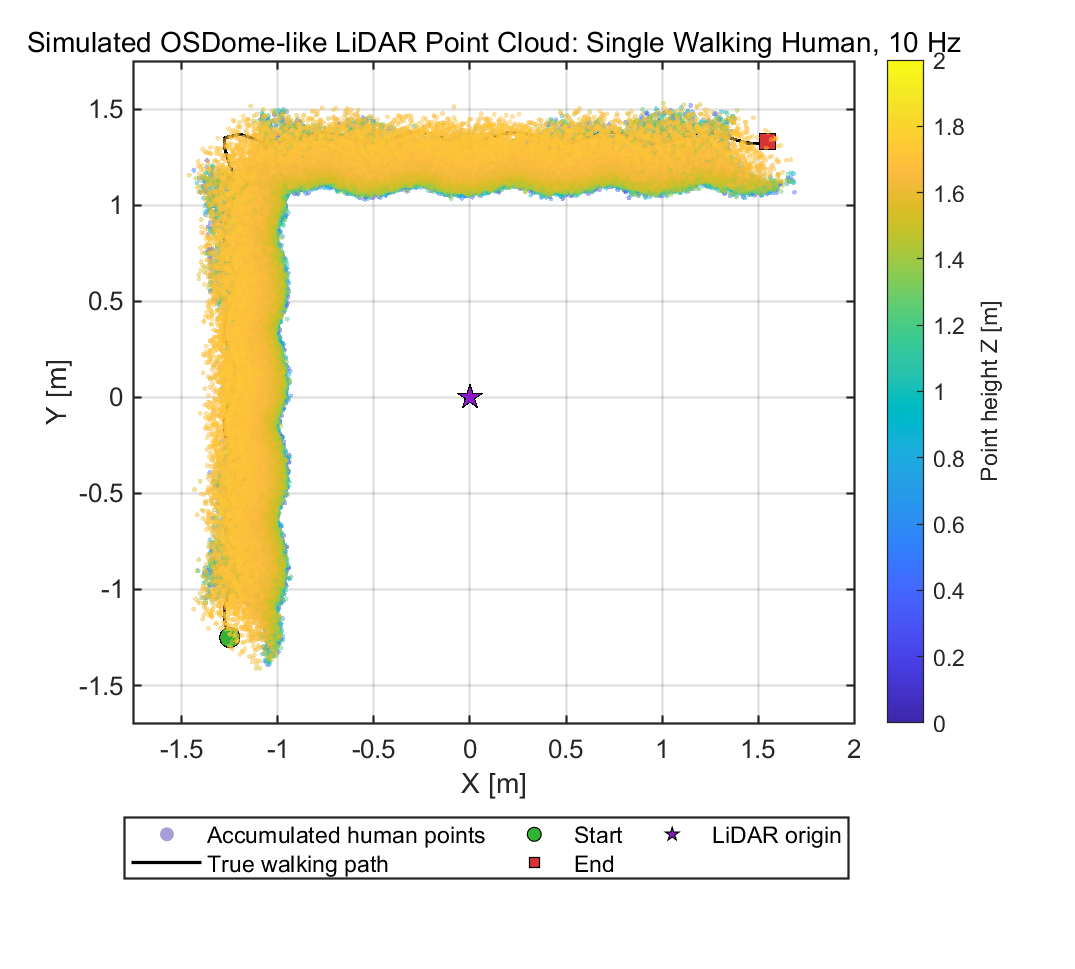
\includegraphics[width=\linewidth]{Figure2.png}

    \vspace{-0.2em}
    \scriptsize (a) Simulated accumulated top-view point cloud.
\end{minipage}
\hfill
\begin{minipage}{0.39\linewidth}
    \centering
    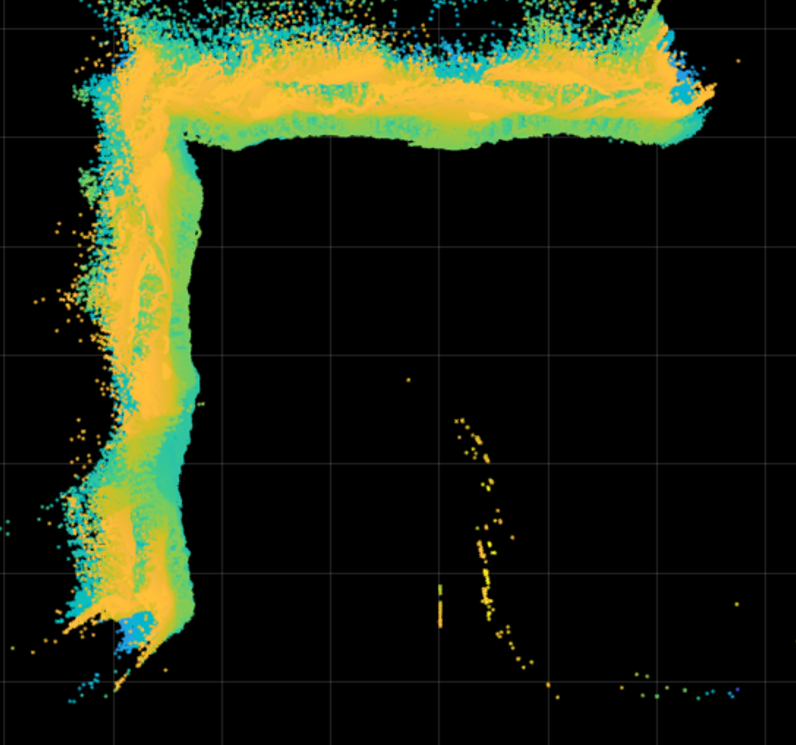
\includegraphics[width=\linewidth]{Figure4.png}

    \vspace{-0.2em}
    \scriptsize (b) Xu's accumulated top-view measurement.
\end{minipage}

\captionof{figure}{Comparison between the simulated and measured accumulated top-view point clouds.}
\label{fig:simulated_measured_accumulated_clouds}
\end{center}

\vspace{0.35em}

As illustrated in Figure~\ref{fig:simulated_measured_accumulated_clouds}, the simulated point cloud (left) is consistent with the real-world measurement (right). Driven by the simulated human trajectory and the integrated point-cloud model, the generated data captures dynamic walking sway, view-dependent density variations (denser on surfaces facing the sensor), and sparsity at extended ranges. Overall, this customized generative model provides an interpretable foundation for preliminary analyses of multi-target clustering, merging, and occlusion handling.

\end{contentbox}
\newpage

\boxitemtitle{2.2 Occlusion: Geometric Shadow Derivation and Ordered Layer}

\begin{contentbox}
\small
\setlength{\abovedisplayskip}{4pt}
\setlength{\belowdisplayskip}{4pt}

\subsection*{Geometric Shadow Derivation}

Occlusion occurs when 1 target enters the geometric shadow cast by another target. In a 2D sectional view, the shadow length $e$ is
\[
e = \frac{h \cdot d}{H-h},
\]
where $H$ is the sensor height, $h$ is the target height, and $d$ is the radial distance from the target to the sensor. In 3D, this length expands into a fan-shaped shadow because of the LiDAR's angular sampling.

\begin{center}
    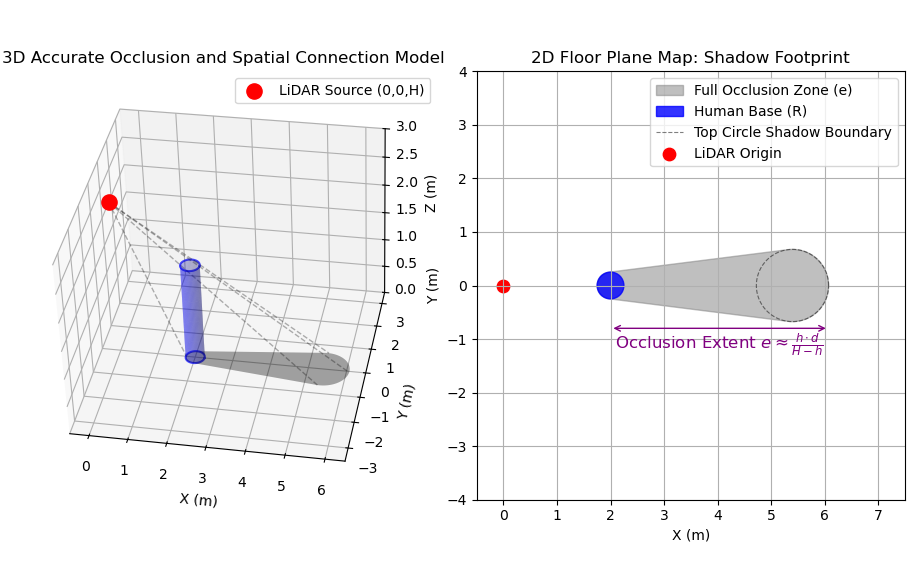
\includegraphics[width=0.9\textwidth]{Figure1.png}
    \vspace{-0.4em}
    \captionof{figure}{Top-down projection and fan-shaped geometric shadow leading to occlusion.}
    \label{fig:shadow_derivation}
\end{center}

\vspace{-0.8em}
\subsection*{Ordered Layers by Distance}

To reduce occlusion complexity, an \textbf{ordered layer} strategy~\cite{advancingMOT2024} can be introduced, where targets are processed from near to far according to their distance from the LiDAR.

\begin{center}
\scriptsize
\setlength{\tabcolsep}{3pt}
\renewcommand{\arraystretch}{0.92}
\begin{tabular}{p{0.28\linewidth} p{0.52\linewidth} p{0.12\linewidth}}
\hline
\textbf{Step} & \textbf{Interpretation} & \textbf{Count} \\
\hline
\textbf{1. Unordered} &
Each target pair has 5 possible states: no occlusion, $T_i$ partially or fully occludes $T_j$, and $T_j$ partially or fully occludes $T_i$. &
$5^{\frac{N(N-1)}{2}}$
\\
\textbf{2. Depth ordered} &
Depth ordering removes back-to-front occlusion, reducing each pair to 3 states: none, partial, and full. &
$3^{\frac{N(N-1)}{2}}$
\\
\textbf{3. Shadow union} &
Targets are scanned from near to far. Each new target is checked against 1 accumulated shadow instead of all previous targets independently. &
$3^{N-1}$
\\
\hline
\end{tabular}
\captionof{table}{Reduction of occlusion-state space using depth ordering and cumulative shadow union.}
\label{tab:occlusion_state_reduction}
\end{center}

For 3 targets, the joint occlusion configurations are reduced from $5^3=125$ in the unordered case to $3^2=9$ after depth ordering and cumulative shadow union. This number describes the occlusion-state space rather than the exact runtime. In implementation, the strategy requires 1 depth-sorting step and 1 near-to-far scan, giving an approximate cost of $O(N\log N + N)$ instead of exhaustive pairwise reasoning.

\end{contentbox}
\newpage

\boxitemtitle{2.3 Merging: A Margin Problem}
\begin{contentbox}
To isolate the merging behavior, a simulation was established under strict ideal conditions: 2 targets, modeled as rounded cylinders with identical radii ($R$), moving at the same speed along a symmetric V-shaped trajectory without mutual occlusion. From a polar-coordinate perspective, occlusion and merging manifest as different spatial phenomena. Occlusion is predominantly a \textit{radial} issue, occurring when targets share a similar angular azimuth ($\theta$) but differ in radial depth ($\rho$). Conversely, merging is a \textit{circumferential} problem when their absolute spatial distance across the horizontal plane becomes too narrow for clustering algorithms like DBSCAN to partition them.

\vspace*{0.2em}
The theoretical clustering failure point is defined by a margin encompassing the physical contact distance, the DBSCAN search radius ($\epsilon$), and a double-sided $3\sigma$ confidence boundary for measurement noise:
\begin{equation}
D_{\text{theory}} = 2R + \epsilon + \Delta_{\text{boundary}} \quad (\text{where } \Delta_{\text{boundary}} = 6\sigma_{\text{noise}}).
\end{equation}


\begin{minipage}[t]{0.42\textwidth}
\vspace{0pt} % Ensures flawless top-alignment of the text block
\small
However, the ray-casting simulation reveals a gap between this theoretical prediction and the actual merge point. Due to the inherent angular sparsity of LiDAR beams along the mutually facing curved surfaces of the cylinders, an ``invisible air buffer'' forms. The algorithm requires the targets to physically "protect" further past $D_{\text{theory}}$ before their sparse boundary point densities overlap sufficiently to form a connected cluster.

\vspace*{0.5em}
Consequently, the merging threshold is more accurately interpreted as a dynamic margin interval $[2R, D_{\text{theory}}]$ rather than a static spatial distance (see Figure~\ref{fig:bubble_effect}). This observation is relevant for tracking robustness: because merging relies on the sparse point distribution along the annular edges, this natural sparsity can delay clustering failure and move the actual merge point closer to the physical contact limit.

\vspace*{0.5em}
By actively exploiting this property and strengthening sparsity, the system can enlarge this ``air buffer''. Such a strategy may act as a geometric protective mechanism under severe spatial proximity.
\end{minipage}%
\hfill
\begin{minipage}[t]{0.55\textwidth}
\vspace{0pt} % Ensures flawless top-alignment of the image graphic
\centering
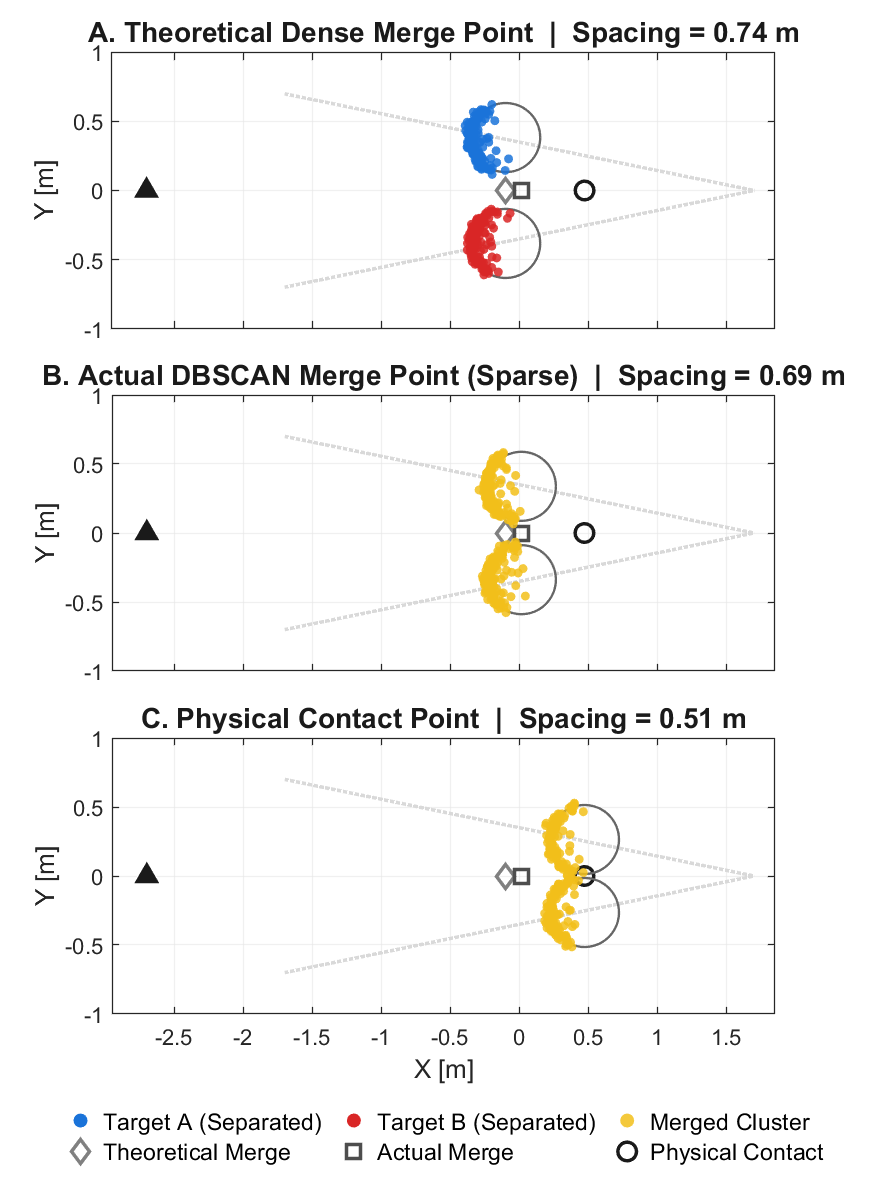
\includegraphics[width=\textwidth]{Figure5.png}
\captionof{figure}{Simulation of the margin gap along a V-shaped trajectory, illustrating the theoretical merge threshold versus the actual sparse-point merge event.}
\label{fig:bubble_effect}
\end{minipage}
\end{contentbox}
\newpage

\boxitemtitle{2.4 3-Voter Mechanism for State Allocation}
\begin{contentbox}
\begin{minipage}[t]{0.57\textwidth}
\vspace{0pt}
In practical tracking, merging and occlusion may occur separately or briefly overlap when targets enter the same high-risk region. Figure~\ref{fig:x_crossing} tests 5 2-person cases: parallel walking, straight X-crossing from 2 LiDAR viewpoints, and X-turning from the same viewpoints. Only the X-turn-bottom case produces ID loss/swap; the KF still keeps an approximate position, but loses reliable turning-direction information after merging. Supplementary ground-truth, calibrated tracking, and 3D accumulated-cloud views are given in AQ4.
\end{minipage}%
\hfill
\begin{minipage}[t]{0.39\textwidth}
\vspace{0pt}
\scriptsize
\renewcommand{\arraystretch}{0.92}
\begin{tabular}{p{0.34\linewidth} p{0.58\linewidth}}
\hline
\textbf{Cue} & \textbf{Meaning} \\
\hline
Red/blue & 2 target identities \\
Yellow & merged or ambiguous points \\
Star & LiDAR position \\
Triangles & occluded centroids; size follows occlusion ratio \\
Lower row & occlusion ratio, density-based quality, and merge flag \\
\hline
\end{tabular}
\end{minipage}

\vspace{-0.2em}
\begin{center}
    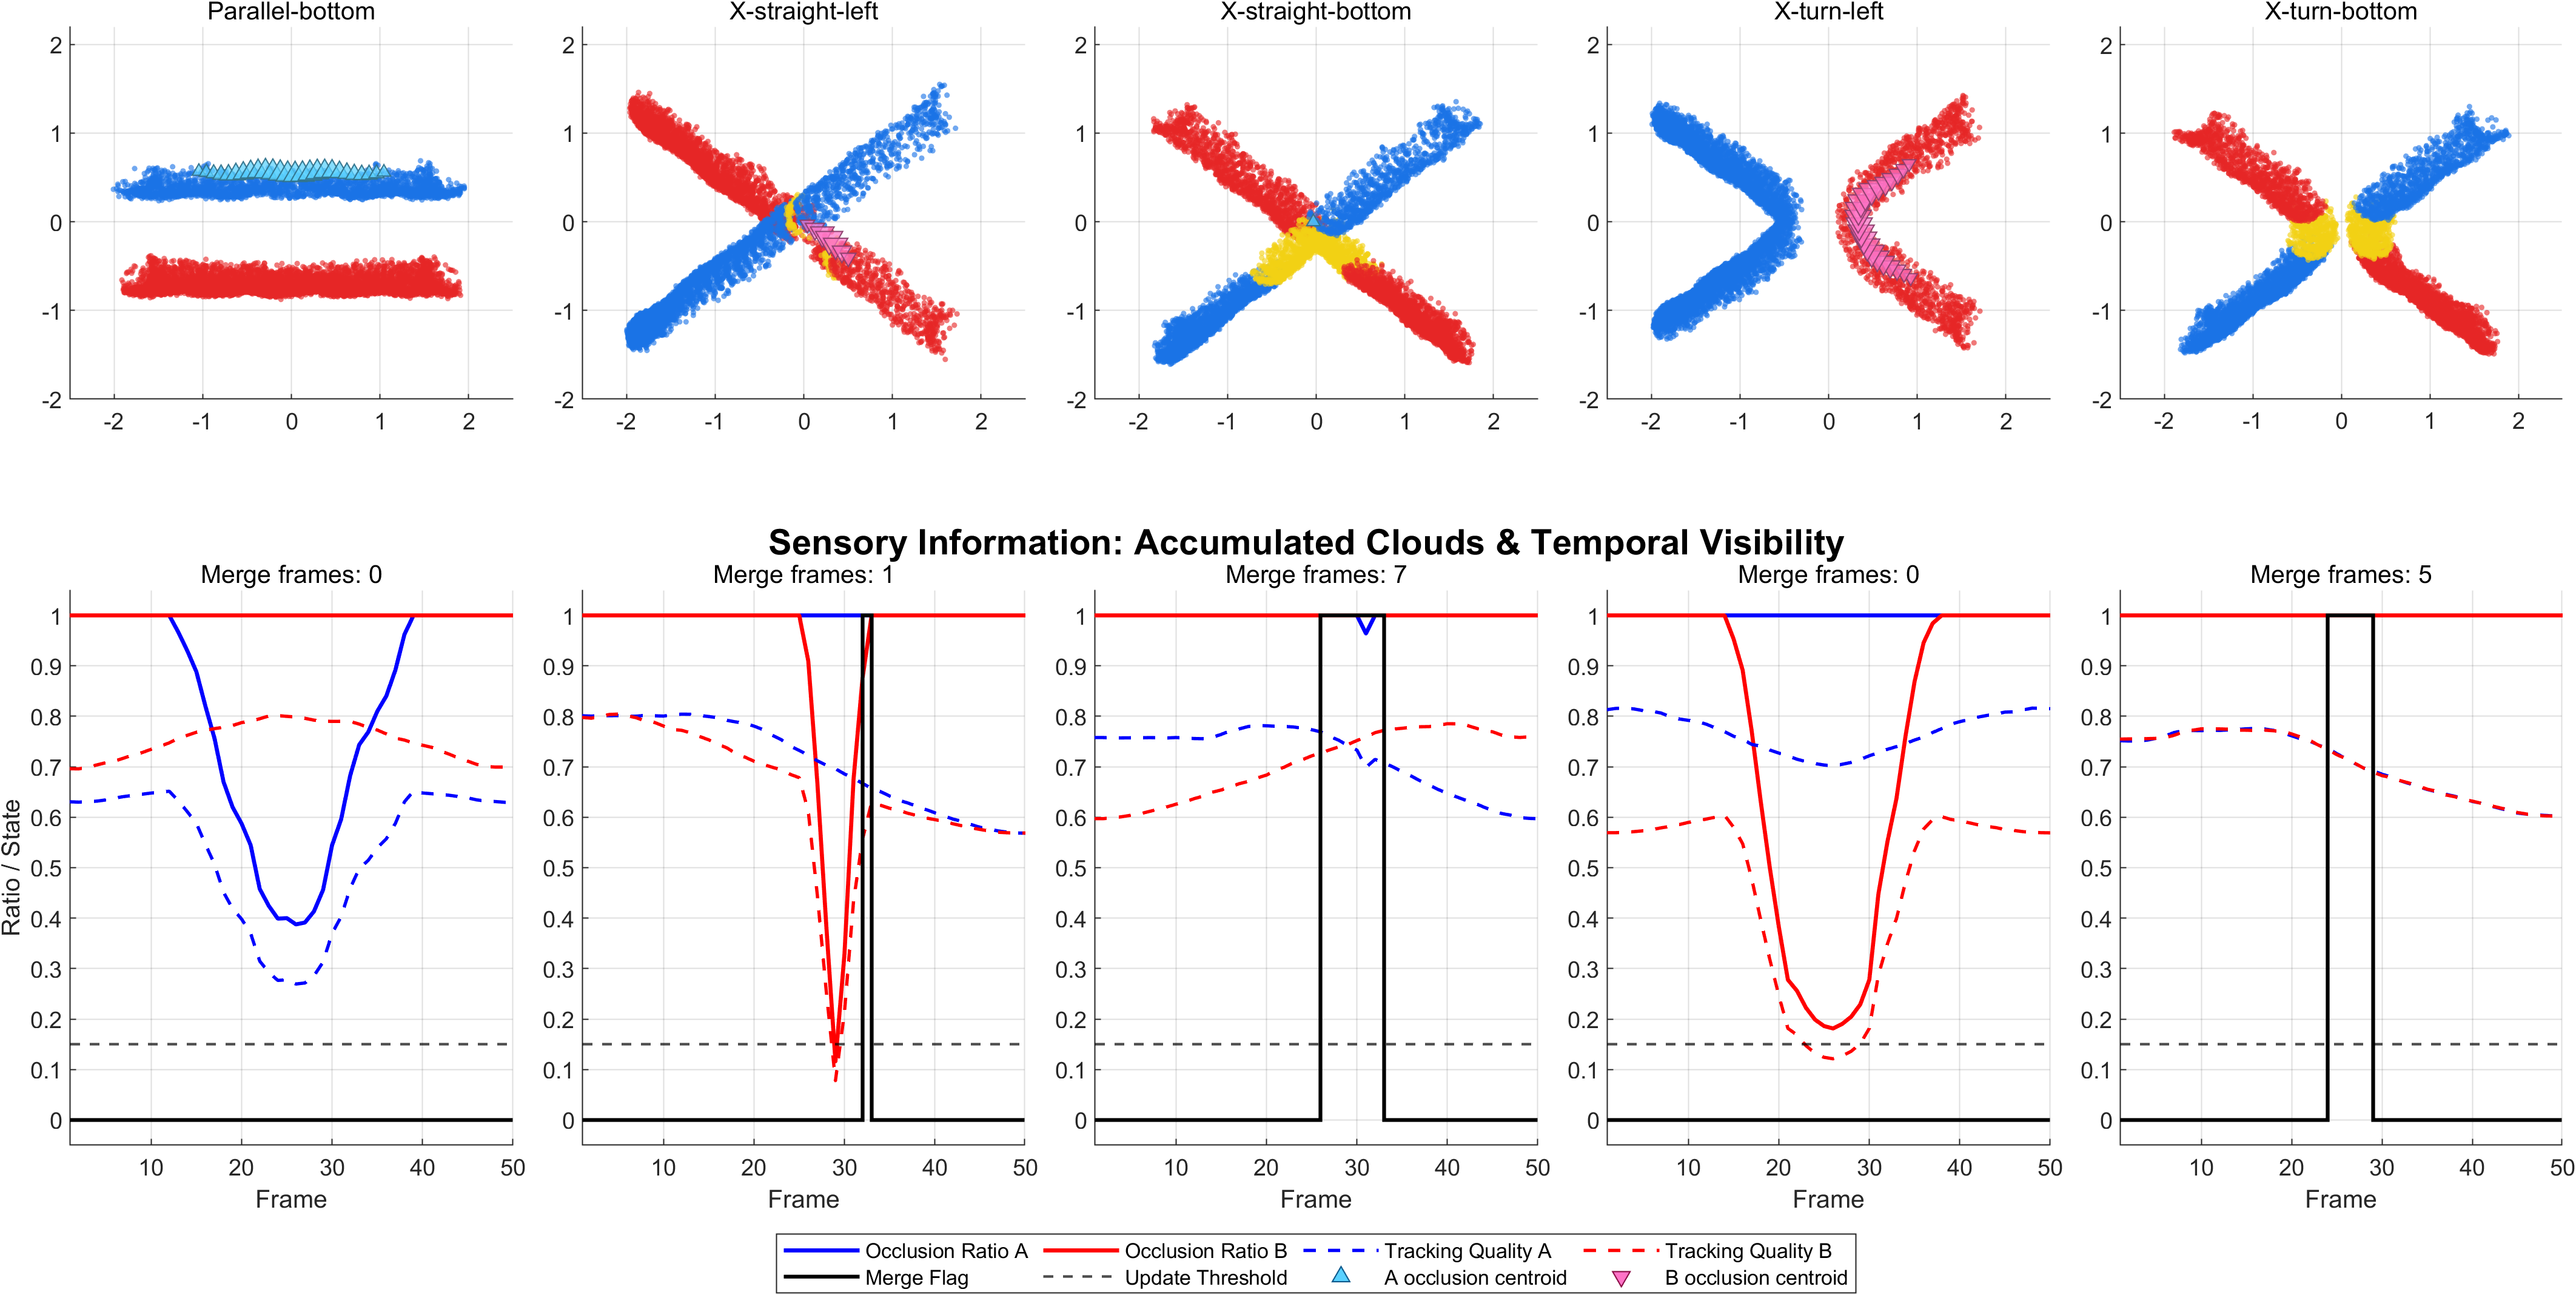
\includegraphics[width=1\textwidth]{Figure9.png}
    \vspace{-0.5em}
    \captionof{figure}{Accumulated point clouds, occlusion ratios, tracking quality, and merge states for the X-shaped 2-person crossing model.}
    \label{fig:x_crossing}
\end{center}

To reduce these ambiguities, a \textbf{3-Voter Mechanism} is proposed for state allocation, such as assigning a ``Wait'' state during unavoidable merging. When spatial coordinates alone are unreliable, 3 independent layers estimate whether 1 cluster contains multiple IDs.

\begin{center}
    \renewcommand{\arraystretch}{1.2}
    \small
    \begin{tabular}{|p{0.25\linewidth}|p{0.68\linewidth}|}
        \hline
        \textbf{Voter Layer} & \textbf{Mechanism and Necessity} \\
        \hline
        \textbf{1. Material and Physical Attributes} &
        Uses LiDAR-intrinsic cues such as reflectivity~\cite{dong2023rliom} and height profiles to distinguish targets with different physical properties. This supports human-robot separation. \\
        \hline
        \textbf{2. Morphology \newline (Shape and Area)} &
        Detects geometric anomalies such as sudden bounding-area expansion or figure-8 contours. Since natural human motion can also change shape, this voter should be validated by the other layers. \\
        \hline
        \textbf{3. Kinematics \newline (Historical Trajectory)} &
        Uses historical velocity and predicted motion to identify high-risk merge zones before spatial clustering fully fails. This helps prepare the state machine in advance. \\
        \hline
    \end{tabular}
    \captionof{table}{The 3 assessment layers of the 3-Voter Mechanism.}
    \label{tab:3_voter}
\end{center}

\vspace*{0.8em}
If the voters confirm that multiple targets are present within 1 cluster, the tracker should avoid immediate ID overwriting. Instead, the uncertain target can be kept in a ``Wait'' state and then recovered after separation using the kinematic and physical voters.
\end{contentbox}

% ==========================================
\chapter{Research Questions}
% ==========================================
\boxitemtitle{RQ1: Multi-Person Tracking}
\begin{contentbox}
\textbf{Can a ceiling-mounted LiDAR reliably separate and track multiple persons, using Yiyun Xu's single-person tracking framework as the baseline?}

\vspace{0.8em}
\textbf{Answer:} Not reliably under all conditions. The single-person framework provides a baseline for foreground segmentation and centroid extraction, but multi-person tracking introduces a new problem: ID persistence. For 1 person, a temporary detection gap mainly affects localization accuracy. For multiple persons, the same gap may cause ID switches, trajectory fragmentation, or false merging.

\vspace{0.6em}
Reliability mainly depends on 2 constraints: 1) the visible point clouds must remain separable enough for clustering, because DBSCAN may collapse multiple persons into 1 cluster once the inter-target distance enters the merging margin; and 2) occlusions must be short enough for the tracker to bridge them using prediction and re-identification. A constant-velocity Kalman filter is a reasonable baseline, but it is not robust enough for sharp turns, crossings, stops, and close interactions.

\vspace{0.6em}
\textit{Conclusion:} A ceiling-mounted LiDAR can support multi-person tracking in sparse indoor scenes, but it cannot be considered reliably scalable without additional data-association logic. The proposed 3-Voter Mechanism, together with stronger filtering models such as EKF, IMM, particle filtering, or GMM-based tracking, should be investigated to preserve IDs during merged or occluded intervals.
\end{contentbox}

\boxitemtitle{RQ2: Mixed-Target Tracking}
\begin{contentbox}
\textbf{Can a ceiling-mounted LiDAR reliably separate and track a heterogeneous mix of multiple targets, specifically persons and robots?}

\vspace{0.8em}
\textbf{Answer:} This case is more promising than human-human tracking because persons and robots usually have more distinguishable LiDAR signatures. Robots often contain metallic or plastic surfaces, regular planar structures, sharp edges, and stable geometric shapes. Human bodies are softer, more irregular, and more time-varying because of clothing, limbs, and gait motion.

\vspace{0.6em}
This case should use 3 main LiDAR-intrinsic cues:
\begin{itemize}[leftmargin=*]
    \item \textbf{Reflectivity:} Different surface materials may generate different reflectivity patterns. R-LIOM shows that reflectivity can be used as an additional LiDAR information channel rather than only as a visualization layer~\cite{dong2023rliom}.
    \item \textbf{Geometry:} Robots are usually more regular in height, width, bounding-box shape, surface-normal distribution, and local roughness, while human point clouds are more deformable.
    \item \textbf{Height:} In a ceiling-mounted setup, height filtering is especially useful. Xu's single-person pipeline already showed that a head-region centroid is more stable than a full-body centroid.
\end{itemize}

\vspace{0em}
The complexity is still limited by target density. Depth ordering and cumulative shadow union can simplify the occlusion reasoning, but dense crowds or many robots in the same small space will still create severe shadows, cluster merging, and ID ambiguity.

\vspace{0.6em}
\textit{Conclusion:} Mixed human-robot tracking has stronger separability than tracking multiple similar human targets, provided that the robot has a stable shape and material signature. The next step should be real indoor testing with both persons and robots, so that target-specific feature fingerprints can be integrated into the Reflectivity Voter, Geometry Voter, and Kinematics Voter.
\end{contentbox}

\newpage

\boxitemtitle{RQ3: Failure Conditions}
\begin{contentbox}
\textbf{Under which conditions does the current tracking system fail?}

\vspace{0.8em}
\textbf{Answer:} The current tracking system is most likely to fail under the following conditions:
\begin{itemize}[leftmargin=*]
    \item \textbf{Target proximity:} When the distance between targets enters the DBSCAN merging margin, multiple targets may be detected as 1 cluster.
    \item \textbf{Mutual occlusion:} A target can temporarily disappear inside another target's geometric shadow, causing missed detections and uncertain ID assignment.
    \item \textbf{Distance-related density loss:} Because of fixed angular resolution, farther targets receive fewer points. This can weaken clustering, centroid estimation, and shape-based classification.
    \item \textbf{Motion-model mismatch:} A constant-velocity prediction can fail when a target turns sharply, stops, accelerates, or intentionally changes direction near an intersection.
    \item \textbf{Environmental noise:} Reflective surfaces, partial visibility, foreground extraction errors, and clothing variation can dominate the centimeter-scale sparsity margin observed in simulation.
\end{itemize}

\textit{Conclusion:} Tracking failure is caused by the interaction of physical target size, DBSCAN parameters, view-dependent sparsity, occlusion ratio, and motion-model mismatch. Therefore, the failure boundary should be treated as a multi-variable condition rather than 1 fixed distance threshold.
\end{contentbox}

\boxitemtitle{RQ4: Data Quality for Evaluation}
\begin{contentbox}
\textbf{Is the resulting trajectory quality sufficient for offline ground-truth evaluation in complex indoor environments?}

\vspace{0.8em}
\textbf{Answer:}
\begin{itemize}[leftmargin=*]
    \item \textbf{For single-person tracking:} Xu's work shows that a ceiling-mounted LiDAR system can provide a reasonably accurate reference trajectory, especially when head-centroid tracking and LiDAR-IMU fusion are used.
    \item \textbf{For multi-target tracking:} The trajectory is not yet sufficient as an absolute ground-truth standard, because ID switches, merged clusters, and trajectory fragmentation become more important than single-centroid localization error.
    \item \textbf{Required evaluation variables:} Effective point-cloud radius, minimum merge distance, point-density decay, occlusion ratio, ID switches, track fragmentation, and recovery time should be added to the evaluation.
    \item \textbf{Practical use:} The trajectory can currently serve as an offline benchmark or qualitative reference, but real multi-target experiments are still required before it can be treated as reliable ground truth.
\end{itemize}
\end{contentbox}

\newpage

% ==========================================
\chapter{Future Work \& Conclusion}
% ==========================================
\begin{sectionintro}{Next Steps}
The next stage should validate the simulation results in measured indoor data and convert the proposed reasoning modules into testable tracking components.
\end{sectionintro}

\begin{contentbox}
\begin{itemize}[leftmargin=*]
    \item \textbf{Empirical field validation:} Test the centimeter-scale sparsity-induced margin in the real laboratory setup and study how sensor noise, clothing, target orientation, and dynamic reflections change the merge threshold.
    \item \textbf{3-Voter implementation:} Implement the Morphology, Kinematics, and Reflectivity voters in the existing pipeline to flag merging events and trigger the Wait/Recover state machine.
    \item \textbf{Advanced filtering models:} Compare standard KF, EKF, IMM, particle filtering, and GMM-based tracking for nonlinear motion and multi-hypothesis recovery during deep occlusion.
    \item \textbf{Human-robot feature testing:} Collect mixed person-robot data and extract reflectivity, height, roughness, and surface-normal fingerprints for target classification.
    \item \textbf{Reinforced sparsity and bubble protection:} Test whether LiDAR-intrinsic masks, multi-feature point weighting, or deliberately strengthened boundary sparsity can reduce the DBSCAN merge distance toward the physical-contact distance without removing valid target returns.
\end{itemize}
\end{contentbox}

\begin{sectionintro}{Final Summary}
The main conclusions are summarized below.
\end{sectionintro}

\begin{contentbox}
\begin{itemize}[leftmargin=*]
    \item \textbf{Research scope:} The project examined the transition from single-target localization to multi-target tracking using a ceiling-mounted LiDAR.
    \item \textbf{Occlusion reasoning:} The fan-shaped shadow model and depth-ordered shadow union reduce mutual occlusion analysis to a near-to-far visibility reasoning problem.
    \item \textbf{Merging behavior:} The simulations indicate that point-cloud sparsity creates a dynamic merging margin rather than 1 fixed merge distance.
    \item \textbf{Tracking strategy:} The proposed 3-Voter Mechanism combines geometry, trajectory history, and reflectivity to support ID preservation when spatial clustering becomes ambiguous.
    \item \textbf{Overall conclusion:} Ceiling-mounted LiDAR can support sparse indoor multi-target tracking, but reliable deployment requires stronger data association, real-data validation, and LiDAR-intrinsic feature use beyond 2D position alone.
\end{itemize}
\end{contentbox}

\newpage
\startappendices

% ==========================================
\chapter{Additional Questions}
% ==========================================
\begin{sectionintro}{Auxiliary Analysis}
This appendix records auxiliary questions that complement the main research scope and preserve additional directions for future work.
\end{sectionintro}

\boxitemtitle{AQ1: Mathematical Derivations of Density Attenuation}
\begin{contentbox}
\setlength{\abovedisplayskip}{3pt}
\setlength{\belowdisplayskip}{3pt}
LiDAR density attenuation can be explained from the ray footprint and from spherical-coordinate scaling. Both views show that fixed angular sampling covers a larger Cartesian region as distance increases.

\vspace{0.25em}
\textbf{1. Area Method with Ground-Plane Projection:}

A LiDAR emits beams at fixed angular increments $\Delta\theta$ and $\Delta\phi$. At distance $d$, the local spherical footprint and its ground-plane projection are
\[
\begin{aligned}
A_s(d) &\approx (d\Delta\theta)(d\Delta\phi)=d^2\Delta\theta\Delta\phi,\\
A_p(d) &\approx A_s(d)\cos\phi=d^2\cos\phi\,\Delta\theta\Delta\phi,\\
\rho_p(d,\phi) &\approx \frac{C}{A_p(d)}
\propto \frac{1}{d^2\cos\phi\,\Delta\theta\Delta\phi}.
\end{aligned}
\]
The $\cos\phi$ term accounts for projecting the spherical ray footprint onto the top-view point-cloud plane; the dominant range term remains $d^2$.

\vspace{0.25em}
\textbf{2. Rigorous Proof via Jacobian Matrix Transformation:}

The same scaling follows from transforming spherical sensor coordinates $(d,\theta,\phi)$ to Cartesian coordinates $(x,y,z)$:
\[
\begin{gathered}
x = d\cos\phi\cos\theta,\quad y = d\cos\phi\sin\theta,\quad z = d\sin\phi,\\
|J_{3D}|=\left|\frac{\partial(x,y,z)}{\partial(d,\theta,\phi)}\right|=d^2\cos\phi.
\end{gathered}
\]
Thus the Cartesian volume element is $dV=(d^2\cos\phi)\,dd\,d\theta\,d\phi$, which matches the projected area reasoning above.

\vspace{0.25em}
\textbf{3. Why a Cylindrical Model Is Not Used:}

A cylindrical model would describe mainly horizontal spreading. In cylindrical coordinates $(r,\theta,z)$, the Jacobian is $r$, so only 1 distance factor appears and the vertical direction has no range-dependent attenuation. This is less consistent with a LiDAR ray pattern, which spreads over both azimuth and elevation. Even when targets are observed on 1 floor and the vertical effect is smaller, point density still depends on object height and elevation angle. Therefore, the spherical/ray-casting model is a better abstraction for ceiling-mounted LiDAR point clouds.

\vspace{0.25em}
\textbf{Insight:}

Both derivations indicate that range-dependent sparsity is mainly governed by $d^2$, with $\cos\phi$ correcting the projection. In a small indoor room, this ideal inverse-square law may appear weaker than $d^{-2}$ because target height, sensor placement, occlusion, and surface visibility also affect the measured point density.
\end{contentbox}

\newpage
\boxitemtitle{AQ2: Nonlinear Complexity of Multi-Target Occlusion}
\begin{contentbox}
Tracking complexity scales nonlinearly with the number of targets. While 2-target occlusion is relatively straightforward, 3 or more targets introduce mutual dependencies and overlapping shadows. If all pairwise occlusion relations are enumerated directly, the number of possible states grows very quickly.

\vspace{0.6em}
\textbf{Core Idea:}

For 1 unordered target pair, there are 5 possible occlusion states: no occlusion, target $T_i$ partially or fully occludes target $T_j$, and target $T_j$ partially or fully occludes target $T_i$. After sorting targets by radial distance from the LiDAR, the farther target cannot physically occlude the closer target. This removes the physically impossible back-to-front cases.

\vspace{0.8em}
\textbf{From Pairwise Tables to Cumulative Shadow:}

\begin{center}
\small
\begin{tabular}{p{0.30\linewidth} p{0.30\linewidth} p{0.30\linewidth}}
\hline
\textbf{Step} & \textbf{Interpretation} & \textbf{State Count} \\
\hline
\textbf{1. Unordered pairwise} &
Each target pair is checked independently. Each pair has 5 possible states. &
$5^{\frac{N(N-1)}{2}}$
\\
\textbf{2. Depth ordered pairwise} &
Depth ordering removes back-to-front occlusion. Each pair is reduced to 3 states: none, partial, and full. &
$3^{\frac{N(N-1)}{2}}$
\\
\textbf{3. Ordered shadow union} &
Targets are scanned from near to far. Each new target is checked only against 1 accumulated shadow, not against all previous targets independently. &
$3^{N-1}$
\\
\hline
\end{tabular}
\end{center}

\vspace{0.9em}
\textbf{Why Cumulative Shadow Reduces the State Space:}

Assume the targets are sorted as $r_1 < r_2 < \cdots < r_N$. The closest target $T_1$ is treated as visible and starts the initial shadow. Then $T_2$ is checked against the shadow of $T_1$, $T_3$ is checked against the accumulated shadow of $T_1$ and $T_2$, and so on. Therefore, only $N-1$ near-to-far visibility checks are needed. Each check has 3 possible outcomes: none, partial, and full. Therefore, the physical state complexity becomes $3^{N-1}$.
\end{contentbox}

\newpage
\boxitemtitle{AQ3: Can Extra LiDAR Features Help Separate Humans and Robots?}
\begin{contentbox}
The point cloud contains more information than 2D position alone. Since this project focuses on LiDAR-only tracking, useful features should be selected from the LiDAR data itself instead of relying on extra cameras or complex calibration.

\vspace{1.0em}
\textbf{Core Idea:}

When 2 targets are close or merged in the 2D plane, extra features such as height, point density, reflectivity, and motion can reduce ambiguity. This is relevant for human-robot tracking because a person and a robot usually have different vertical sizes, surface regularity, material reflectivity, and motion patterns.

\vspace{0.8em}
\textbf{Useful Feature Groups:}
\begin{itemize}[leftmargin=*]
    \item \textbf{Geometry Features:} Height, vertical extent, width, bounding-box size, and head region.
    \item \textbf{Material Features:} Reflectivity distribution, intensity stability, and material-dependent return patterns.
    \item \textbf{Visibility Features:} Visible point ratio, point density, shadow area, and point loss.
    \item \textbf{Motion Features:} Velocity, acceleration, smoothness, turning behavior, and gait oscillation.
\end{itemize}

\vspace{0.8em}
\textbf{Reflectivity as a Pseudo-Visual Cue:}

Reflectivity can be treated as an independent LiDAR-intrinsic feature rather than only a visualization value. Ouster sensors provide 8-bit reflectivity/intensity information, and R-LIOM shows that corrected reflectivity can be converted into grayscale pseudo-visual images~\cite{dong2023rliom}. This means that a LiDAR-only system can obtain camera-like cues, such as horizontal extent, surface pattern, and material contrast, without adding a camera.

For mixed human-robot tracking, this channel can be used in 3 compact ways: 1) reflectivity can be combined with height filtering to suppress unreliable ground reflections and emphasize target-level returns; 2) reflectivity descriptors can be combined with KNN-style neighborhood matching or state estimation to improve target consistency when geometry is ambiguous; and 3) corrected reflectivity can be mapped into grayscale pseudo-images, allowing lightweight visual-style features to support classification and re-identification. Therefore, reflectivity is a useful candidate for the Reflectivity Voter, especially when close targets have similar shapes but different materials.
\end{contentbox}

\newpage
\boxitemtitle{AQ4: Supplementary Details for the X-Crossing Experiment}
\begin{contentbox}
This appendix item provides supplementary views for the X-crossing experiment in Section 2.4. Figure~\ref{fig:aq4-tracking-model-overview} shows the ground-truth motion models, calibrated KF tracks, and RMSE values for the 5 test cases. The parallel case uses 2 identical object models with the same speed. In columns 2 and 3, the targets move straight through the X-shaped crossing; target A waits for about $1~\mathrm{s}$, so the closest distance remains about $0.52~\mathrm{m}$, still larger than $2R=0.50~\mathrm{m}$. In columns 4 and 5, the targets turn near the crossing focus with centripetal acceleration and a short circular arc.

\vspace{-0.35em}
\begin{center}
    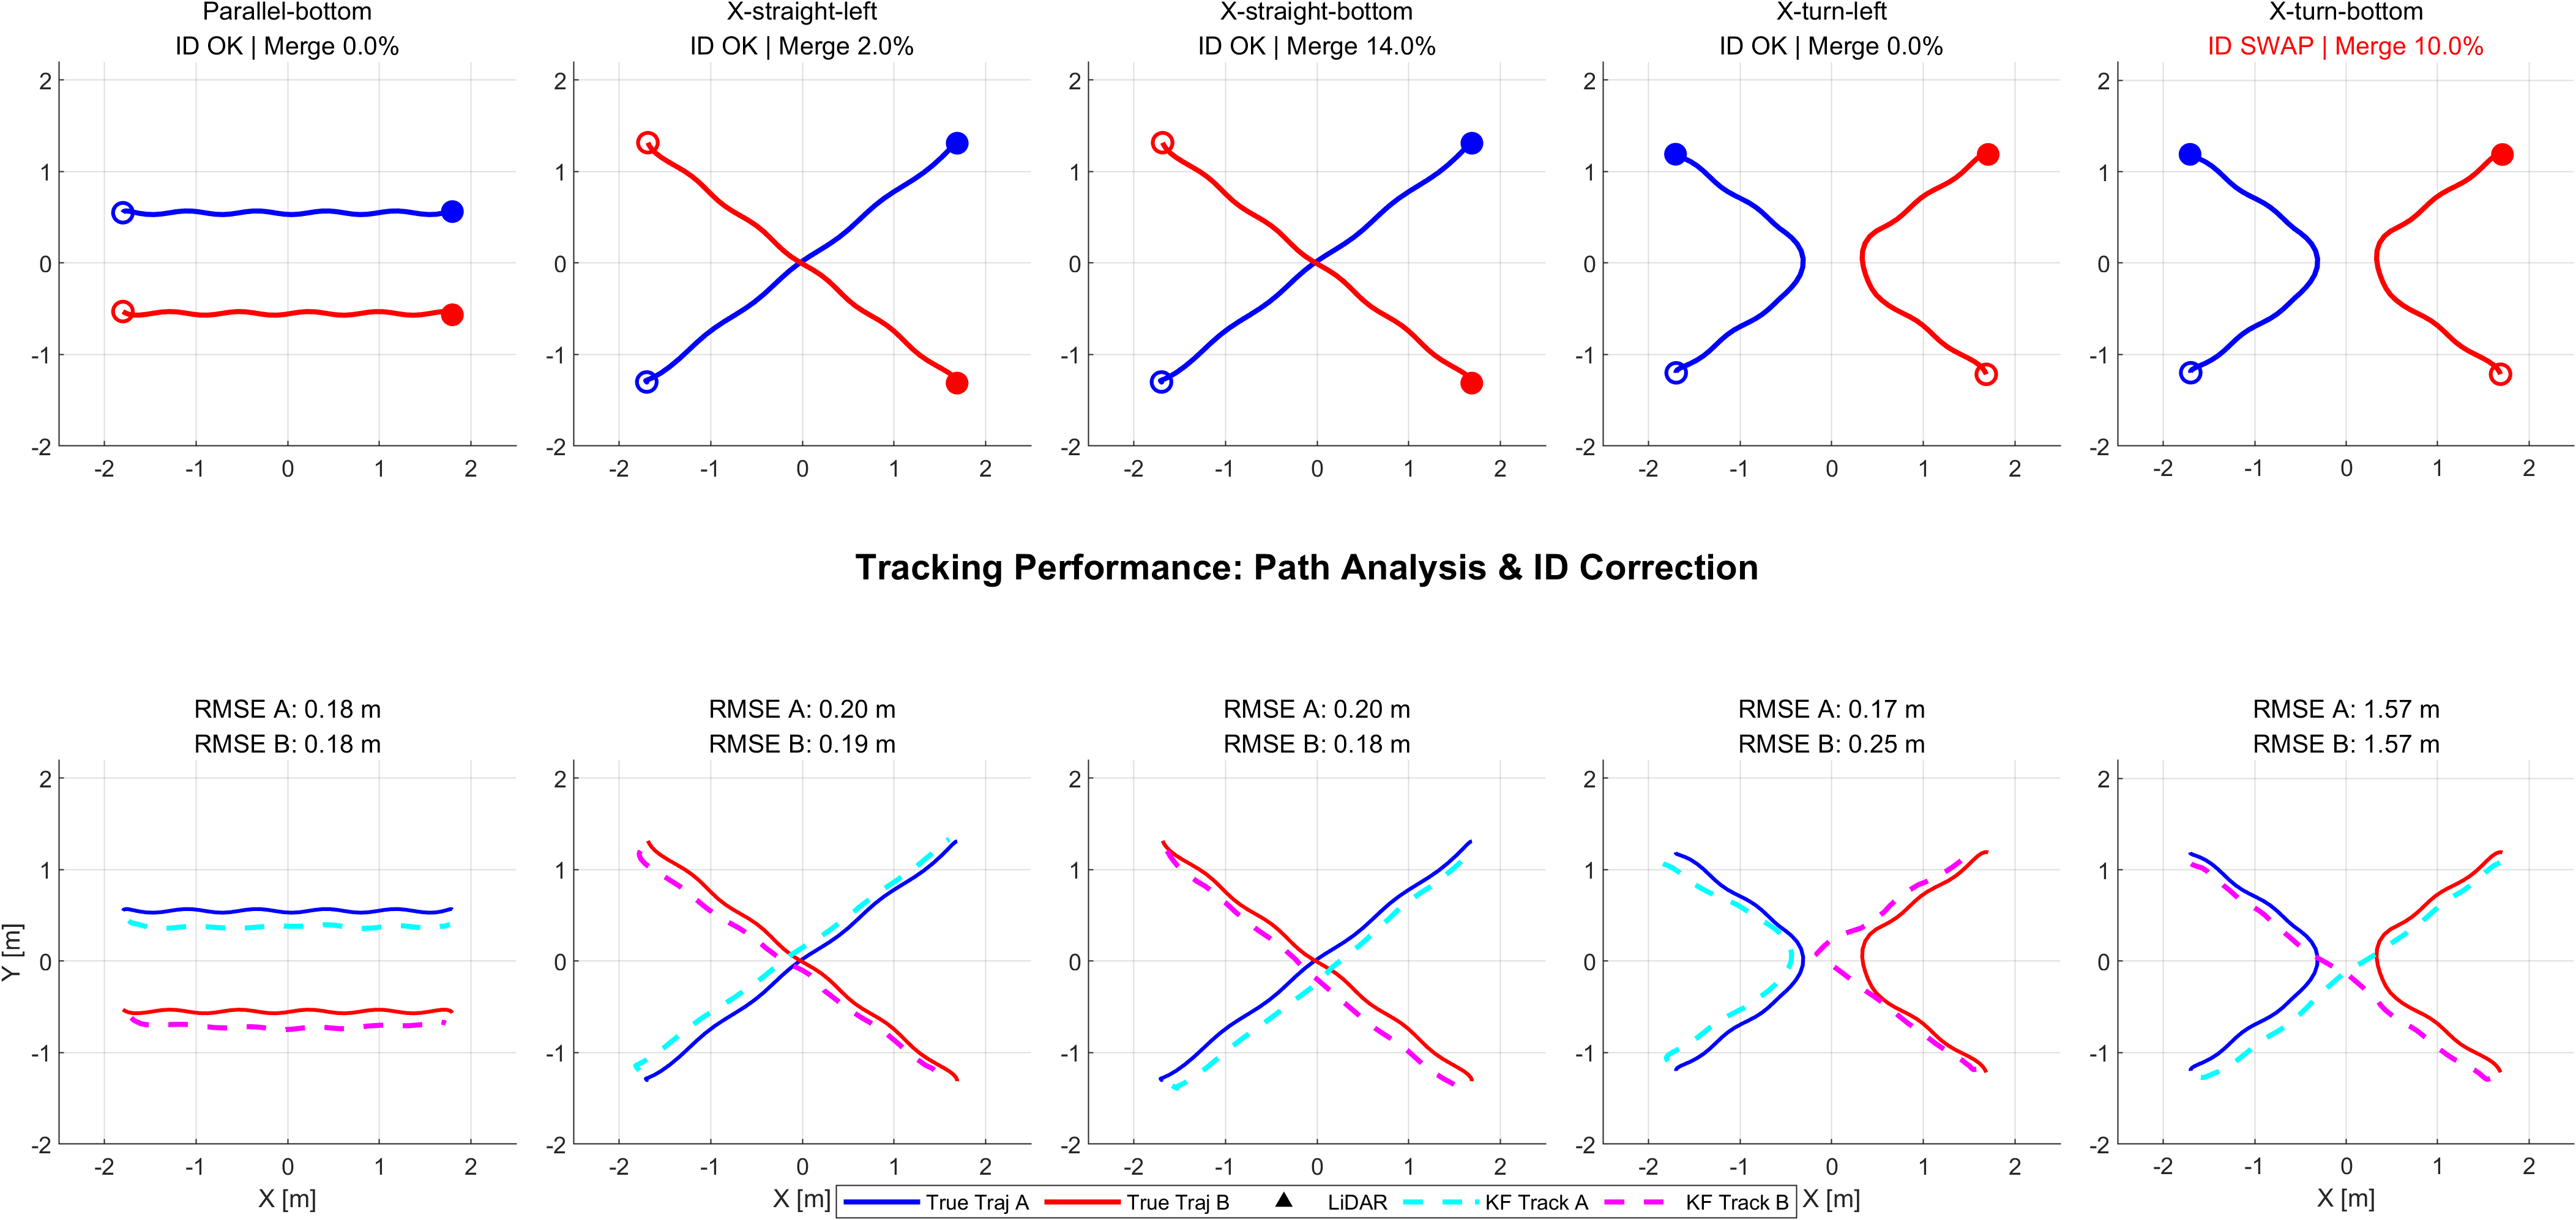
\includegraphics[width=0.88\linewidth]{Figure8.png}
    \captionof{figure}{Ground-truth trajectories, calibrated KF trajectories, and RMSE values for the X-crossing test cases.}
    \label{fig:aq4-tracking-model-overview}
\end{center}
\vspace{-0.55em}

The dashed prediction lines usually lean toward the LiDAR-observed side of the point cloud, because the sensor-facing side has denser measurements and contributes more strongly to the estimated trajectory.

\vspace{-0.35em}
\begin{center}
    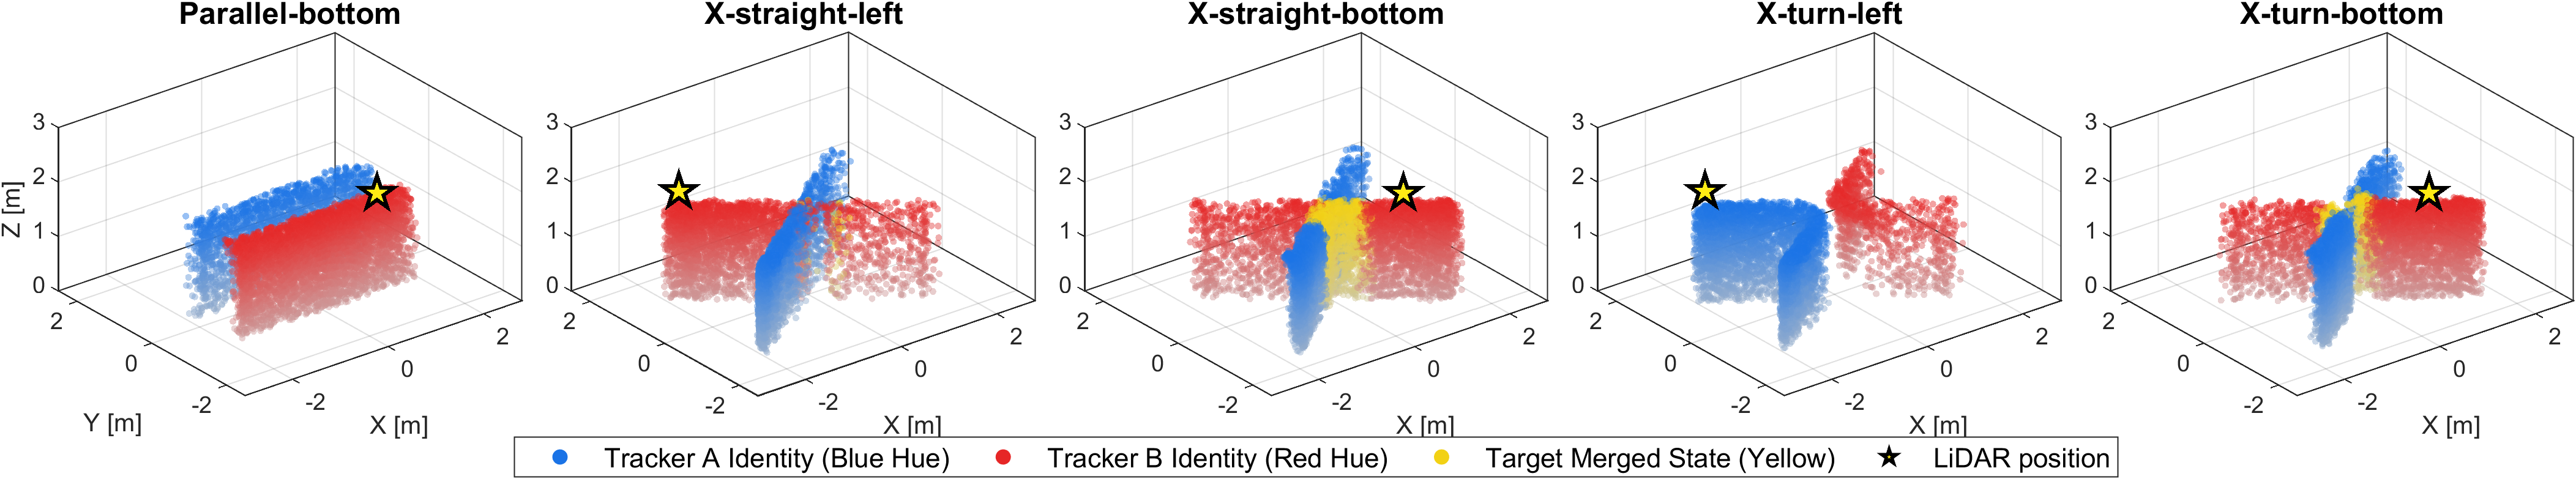
\includegraphics[width=0.88\linewidth]{Figure10.png}
    \captionof{figure}{Oblique 3D accumulated point-cloud views for the X-crossing cases.}
    \label{fig:aq4-kf-stress-summary}
\end{center}
\vspace{-0.55em}

Figure~\ref{fig:aq4-kf-stress-summary} gives an oblique 3D accumulated point-cloud view, making the 2 walking trajectories and LiDAR-view dependence easier to observe. The same motion model can produce different tracking outcomes from different LiDAR viewpoints, depending on whether merged points remain visible or occlusion removes too many points.

The main conclusion is that turning inside a high-risk crossing region can make a simple linear filter fail, especially after merging removes direction information. Future models should therefore consider EKF, IMM, particle filtering, or GMM-based tracking, together with stronger target fingerprints such as $Z$-axis height and reflectivity. Merging and occlusion are physically different failure modes, but they can overlap during short high-risk intervals; stable features from non-merged and non-occluded frames can support trajectory prediction during these ambiguous periods.
\end{contentbox}

\newpage
\boxitemtitle{AQ5: Can an Elliptical Human Model Improve Multi-Target Boundary Analysis?}
\begin{contentbox}
In the current simulation, each person is simplified as a circular or cylindrical object. This provides a baseline. However, a real human body is not perfectly circular in the horizontal plane. From a top-view LiDAR perspective, the human footprint is usually closer to an anisotropic shape with different length and width.

\vspace{1.0em}
\textbf{Core Idea:}

Instead of using 1 fixed radius in all directions, the human target can be represented by an elliptical effective boundary whose orientation is inferred from 2 coupled cues: the LiDAR-facing visibility direction and the target's motion direction. This is important for LiDAR-only tracking because ray-casting mainly samples the visible side of the body, so a person may appear as a crescent-like or partial elliptical point cloud rather than a complete circle or square. Therefore, the model should not only fit an ellipse, but also extract orientation cues from this anisotropic, incomplete local structure and recover a more reliable target direction and boundary during merging and occlusion.

\vspace{0.8em}
\textbf{Main Challenges:}
\begin{itemize}[leftmargin=*]
    \item \textbf{Orientation Ambiguity:} The ellipse requires direction information, but the true body heading cannot always be reliably observed from 1 LiDAR frame.
    \item \textbf{Point-Cloud Degradation:} During merging, occlusion, or sparse sampling at long distance, the cluster shape may be incomplete, making the fitted ellipse unstable.
\end{itemize}
\end{contentbox}

\newpage
\boxitemtitle{AQ6: Can the ``Bubble Effect'' be Leveraged as an Active Strategy to Prevent Cluster Merging?}
\begin{contentbox}
The view-dependent ``Bubble Effect'' can be used as a possible strategy for delaying DBSCAN cluster merging. When the point cloud becomes sparse near the contact area between 2 targets, the low-density gap can help the tracker keep 2 IDs separated for a longer time.

\vspace{0.8em}
\textbf{1. Natural Bubble Buffer}
\\
The natural bubble buffer appears when 2 targets approach each other but the LiDAR returns near their facing boundaries remain sparse. As shown in Figure~\ref{fig:aq6-natural-bubble}, DBSCAN depends on local point density, controlled by the search radius $\epsilon$ and the minimum neighbor count $MinPts$. If the gap between the 2 point clouds is still sparse, the clusters may stay separated even when the physical targets are close. This delays the ID merge and creates a short protection zone before contact.

\begin{center}
    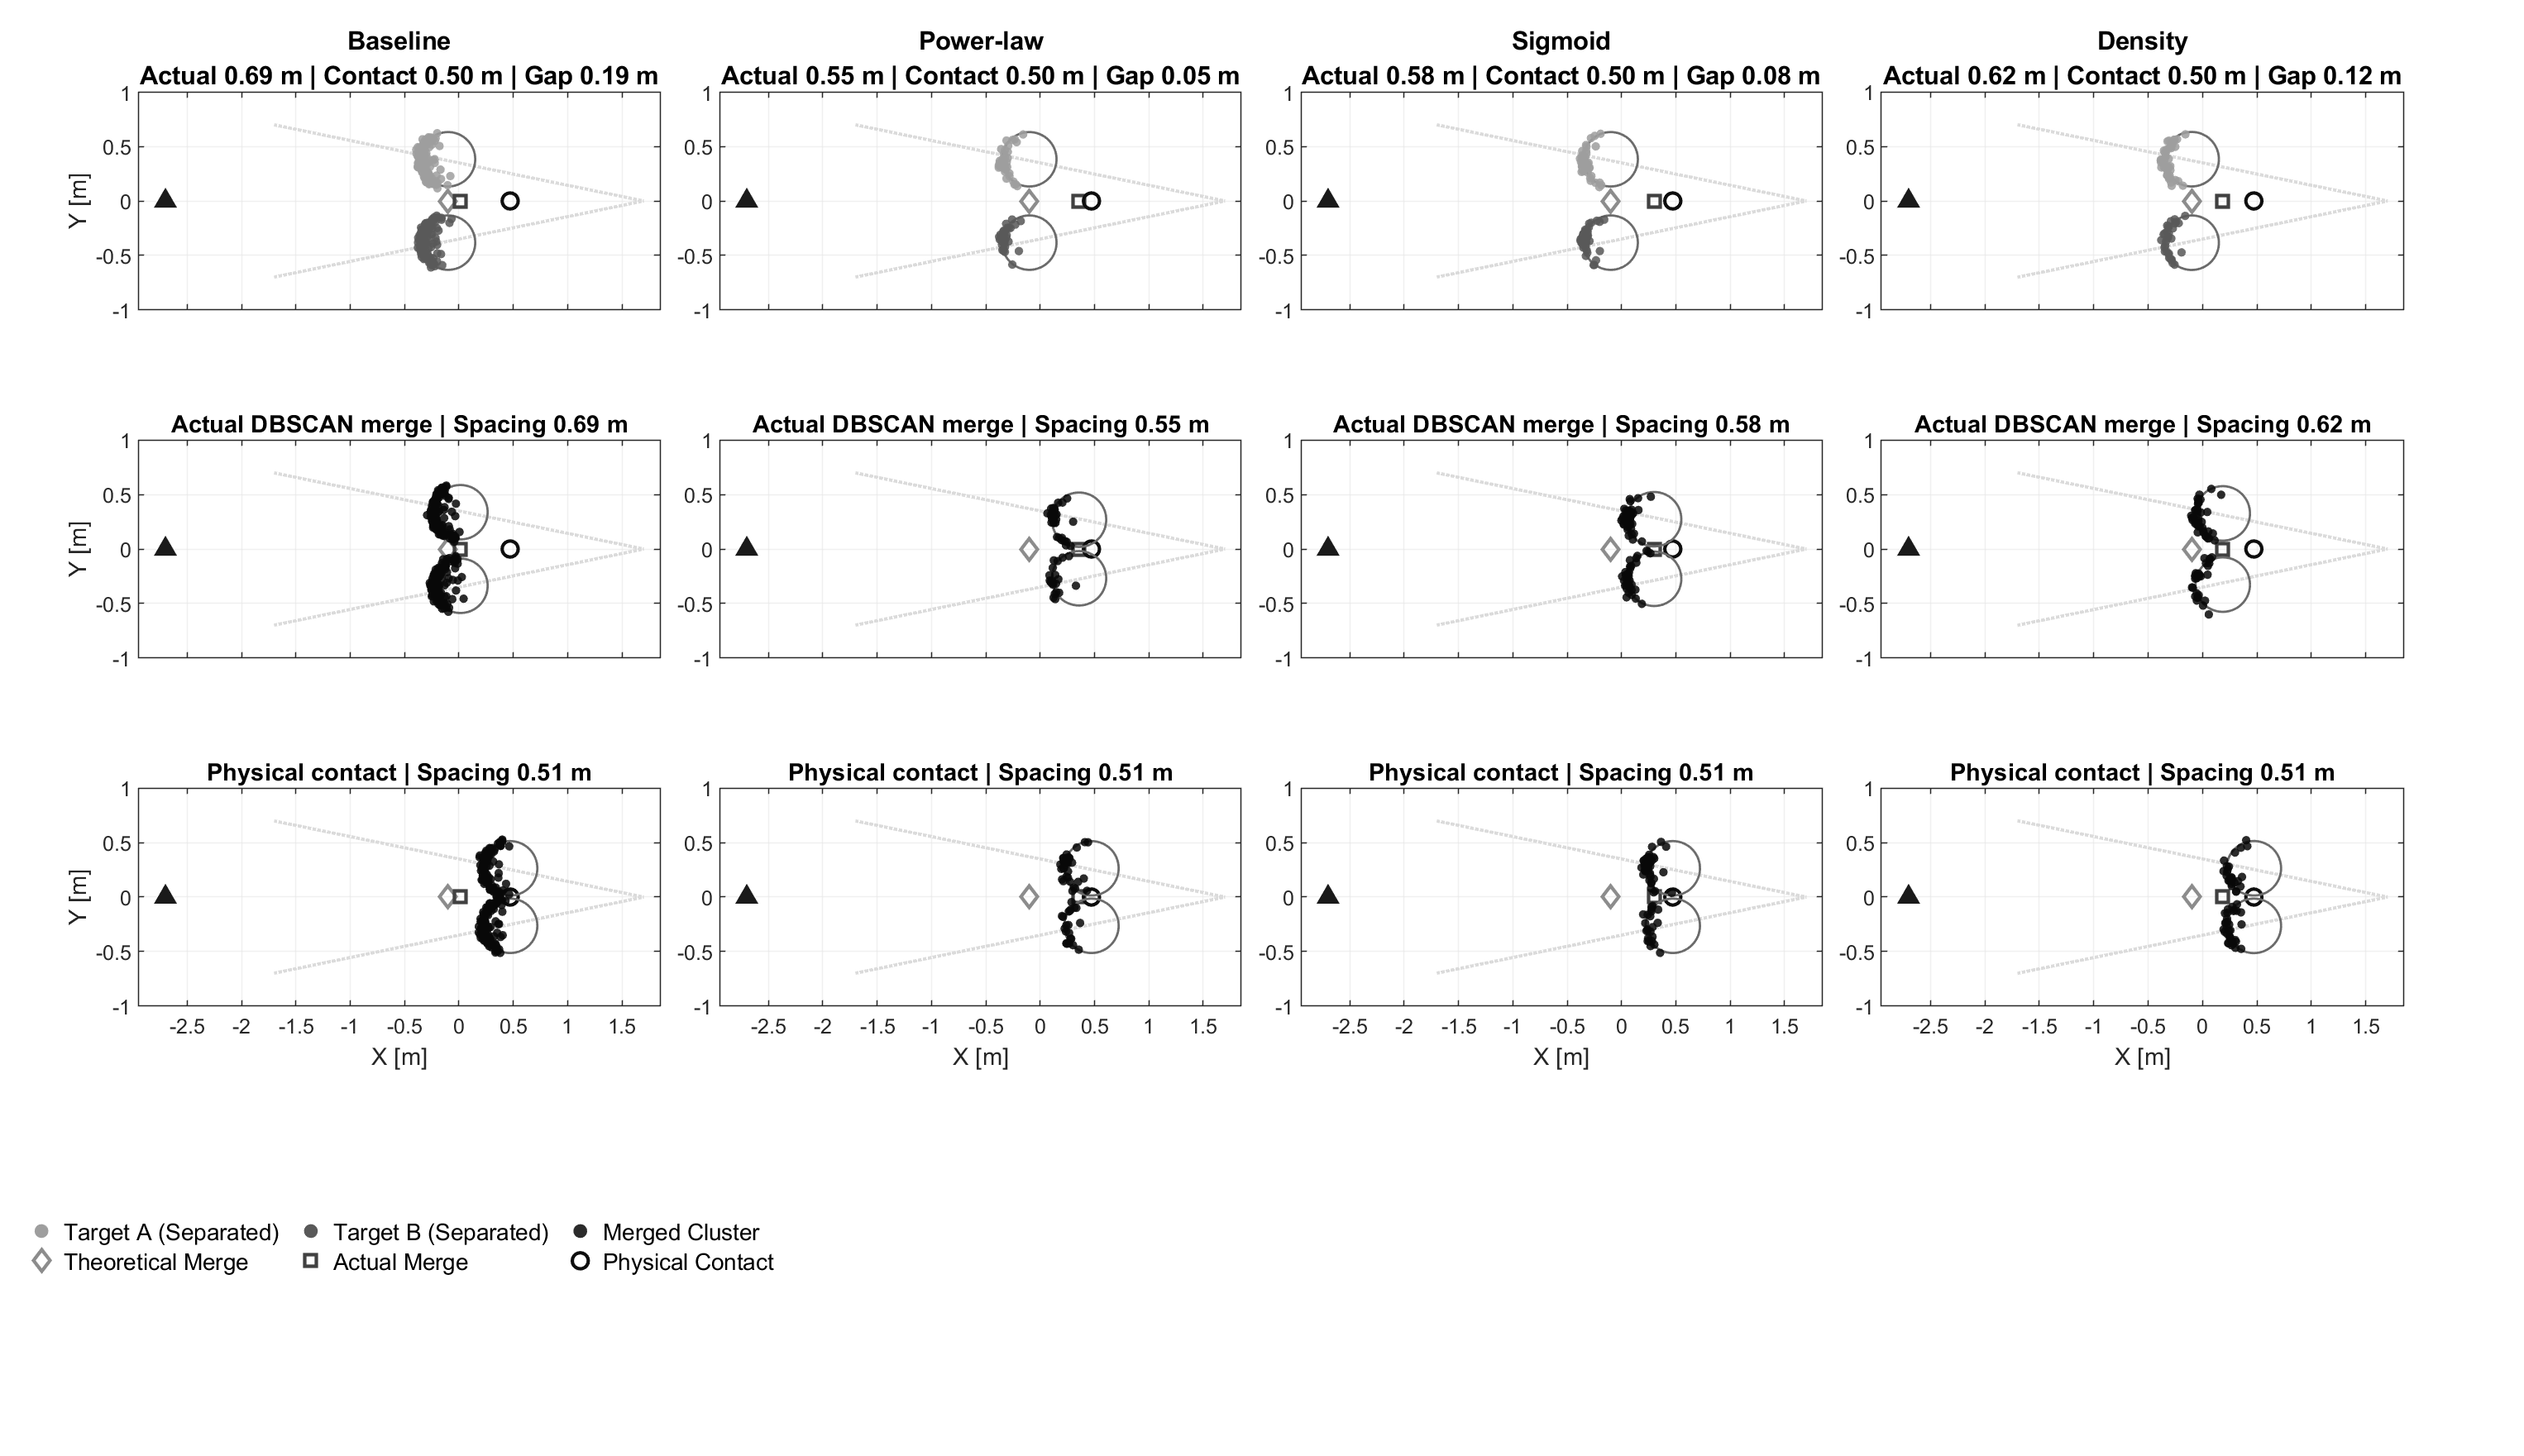
\includegraphics[width=0.95\linewidth]{Figure6.png}
    \captionof{figure}{Natural bubble buffer caused by sparse points near the merging boundary.}
    \label{fig:aq6-natural-bubble}
\end{center}

\vspace{0.8em}
\textbf{2. 3 Tested Buffer Models}
\\
The anisotropy test compares 1 baseline with 3 buffer-strengthening models. The baseline is the normal range-decay simulation and is used only for comparison. The 3 active models shown in Figure~\ref{fig:aq6-engineered-buffer} are \textbf{Power-law}, \textbf{Sigmoid}, and \textbf{Density}.

Let $m_0$ be the minimum keep probability. Let $s \in [0,1]$ be the face score, where larger $s$ means that a point faces the LiDAR more directly.

\begin{itemize}[leftmargin=*]
    \item \textbf{Power-law face-score model.} This method uses the face score and raises it to a power. Boundary points with low face score are kept with lower probability:
    \begin{equation}
    P_{\text{keep}} = m_0 + (1 - m_0)s^p
    \end{equation}

    \item \textbf{Sigmoid face-score model.} This method uses the same face score but applies a soft threshold. Points below the threshold are reduced more strongly, while points above it are mostly preserved:
    \begin{equation}
    P_{\text{keep}} = m_0 + (1 - m_0)\frac{1}{1+\exp[-k_s(s-s_0)]}
    \end{equation}

    \item \textbf{Density self-reinforcement model.} This method uses local point density from neighbor distance. For each point, $d_{k_n}$ is the distance to its $k_n$-th nearest neighbor, and $\rho_{\text{norm}}$ is the normalized density score:
    \begin{equation}
    \rho = \frac{1}{d_{k_n}+\varepsilon}, \qquad
    P_{\text{keep}} = m_0 + (1 - m_0)\rho_{\text{norm}}^q
    \end{equation}
\end{itemize}

\begin{table}[h!]
\centering
\small
\renewcommand{\arraystretch}{1.2}
\begin{tabular}{llcc}
\hline
\textbf{Model} & \textbf{Parameter} & \textbf{Meaning} & \textbf{Value} \\ \hline
\textbf{Power-law} & $p$ & face-score power & $4$ \\
                  & $m_0$ & minimum keep probability & $0.165$ \\ \hline
\textbf{Sigmoid}  & $s_0$ & face-score threshold & $0.64$ \\
                  & $k_s$ & threshold sharpness & $20$ \\
                  & $m_0$ & minimum keep probability & $0.18$ \\ \hline
\textbf{Density}  & $k_n$ & neighbor index for density & $9$ \\
                  & $q$ & density-score power & $4$ \\
                  & $m_0$ & minimum keep probability & $0.16$ \\ \hline
\end{tabular}
\caption{Parameters used by the Power-law, Sigmoid, and Density buffer models.}
\label{tab:aq6_parameters}
\end{table}

Figure~\ref{fig:aq6-engineered-buffer} compares the baseline with the 3 active models. The result shows consistent behavior under the tested settings and random structural noise ($\sigma = 0.015\text{ m}$). Because the plotted gap is the distance between the actual DBSCAN merge point and physical contact, a lower gap is better: it means the cluster merge is delayed until the targets are closer to real contact.

\begin{center}
    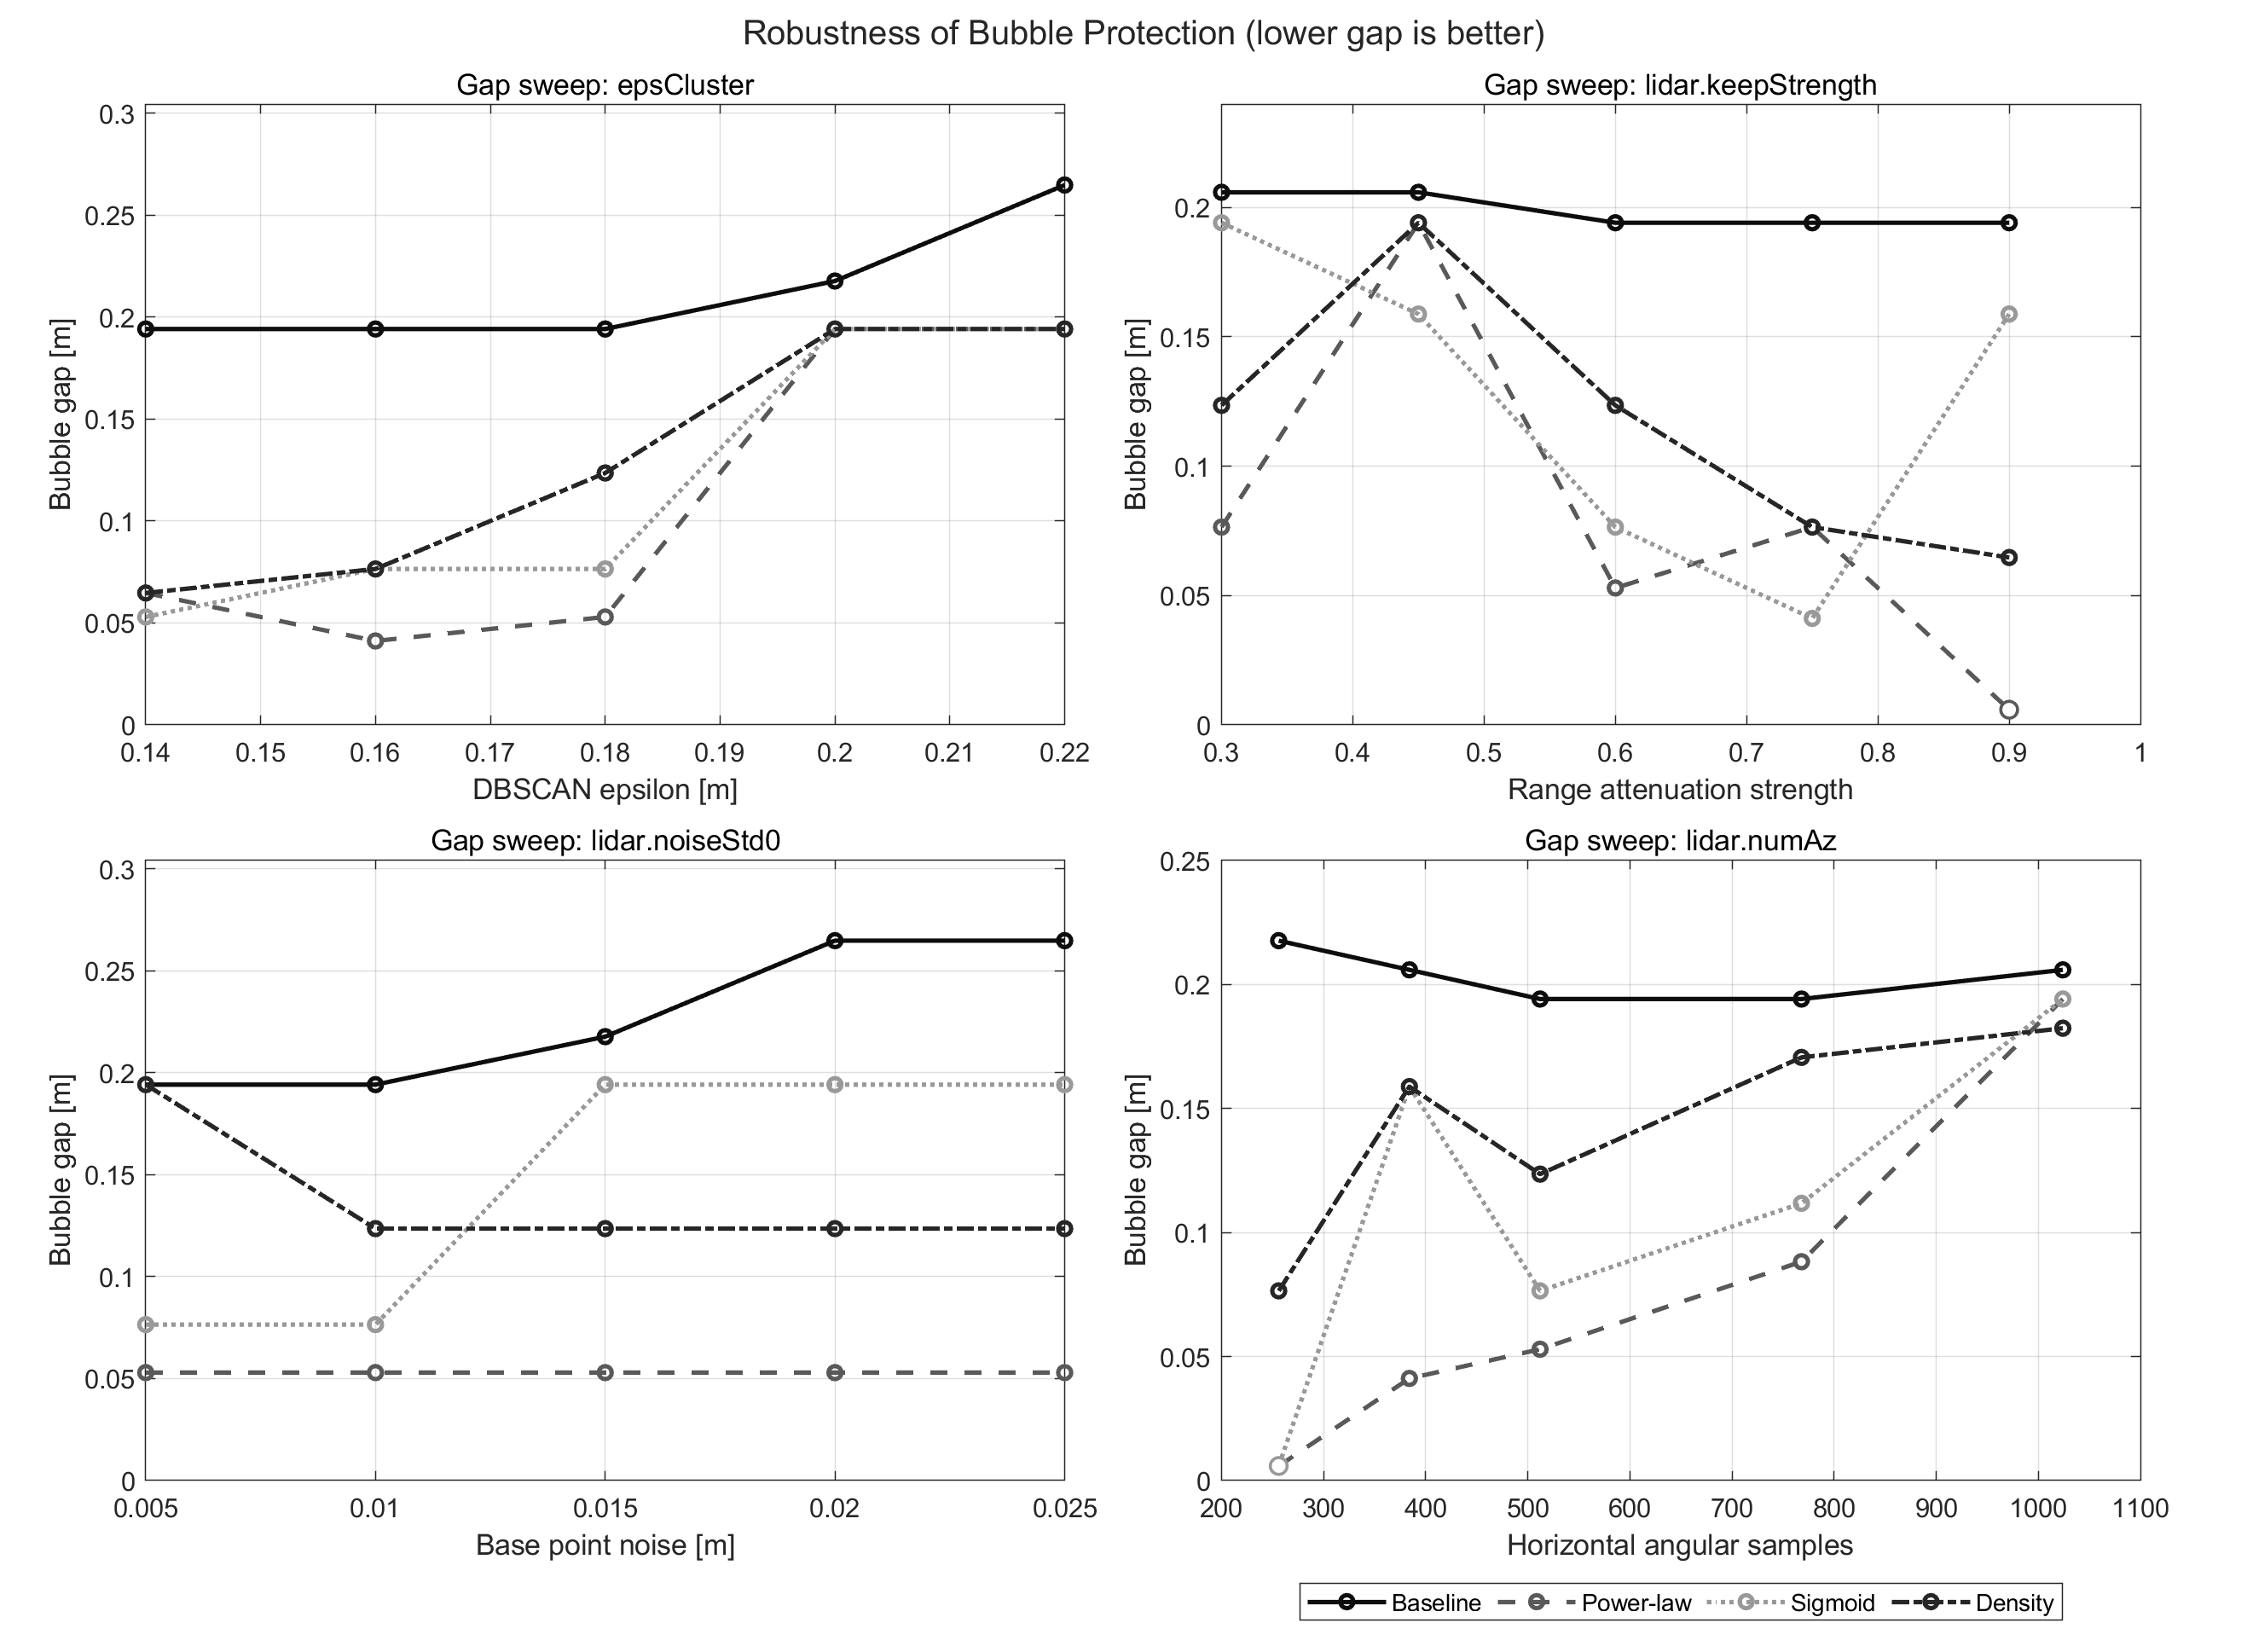
\includegraphics[width=0.95\linewidth]{Figure7.png}
    \captionof{figure}{Bubble-buffer comparison for Baseline, Power-law, Sigmoid, and Density models.}
    \label{fig:aq6-engineered-buffer}
\end{center}

Figures~\ref{fig:aq6-baseline-powerlaw-detail}--\ref{fig:aq6-merge-zoom-detail} provide enlarged views of the same AQ6 experiment rather than separate experiments. These figures show local details of the Figure~\ref{fig:aq6-engineered-buffer} result. Figure~\ref{fig:aq6-baseline-powerlaw-detail} compares the baseline and Power-law models at the theoretical merge point, actual DBSCAN merge point, and physical-contact point. The baseline merges at a spacing of about $0.69~\mathrm{m}$, while the Power-law model delays the actual merge to about $0.55~\mathrm{m}$, much closer to the $0.50~\mathrm{m}$ contact distance.

\vspace{0.8em}
\textbf{3. Practical Meaning}
\\
These models suggest that a tracking pipeline can delay premature merging by adjusting point keep probabilities before clustering. The method does not require extra hardware, but real room data are still needed because clutter, reflections, and different materials may change the bubble shape. The next step is to tune the parameters on measured data and check whether ID separation improves without losing valid target points.

\begin{center}
    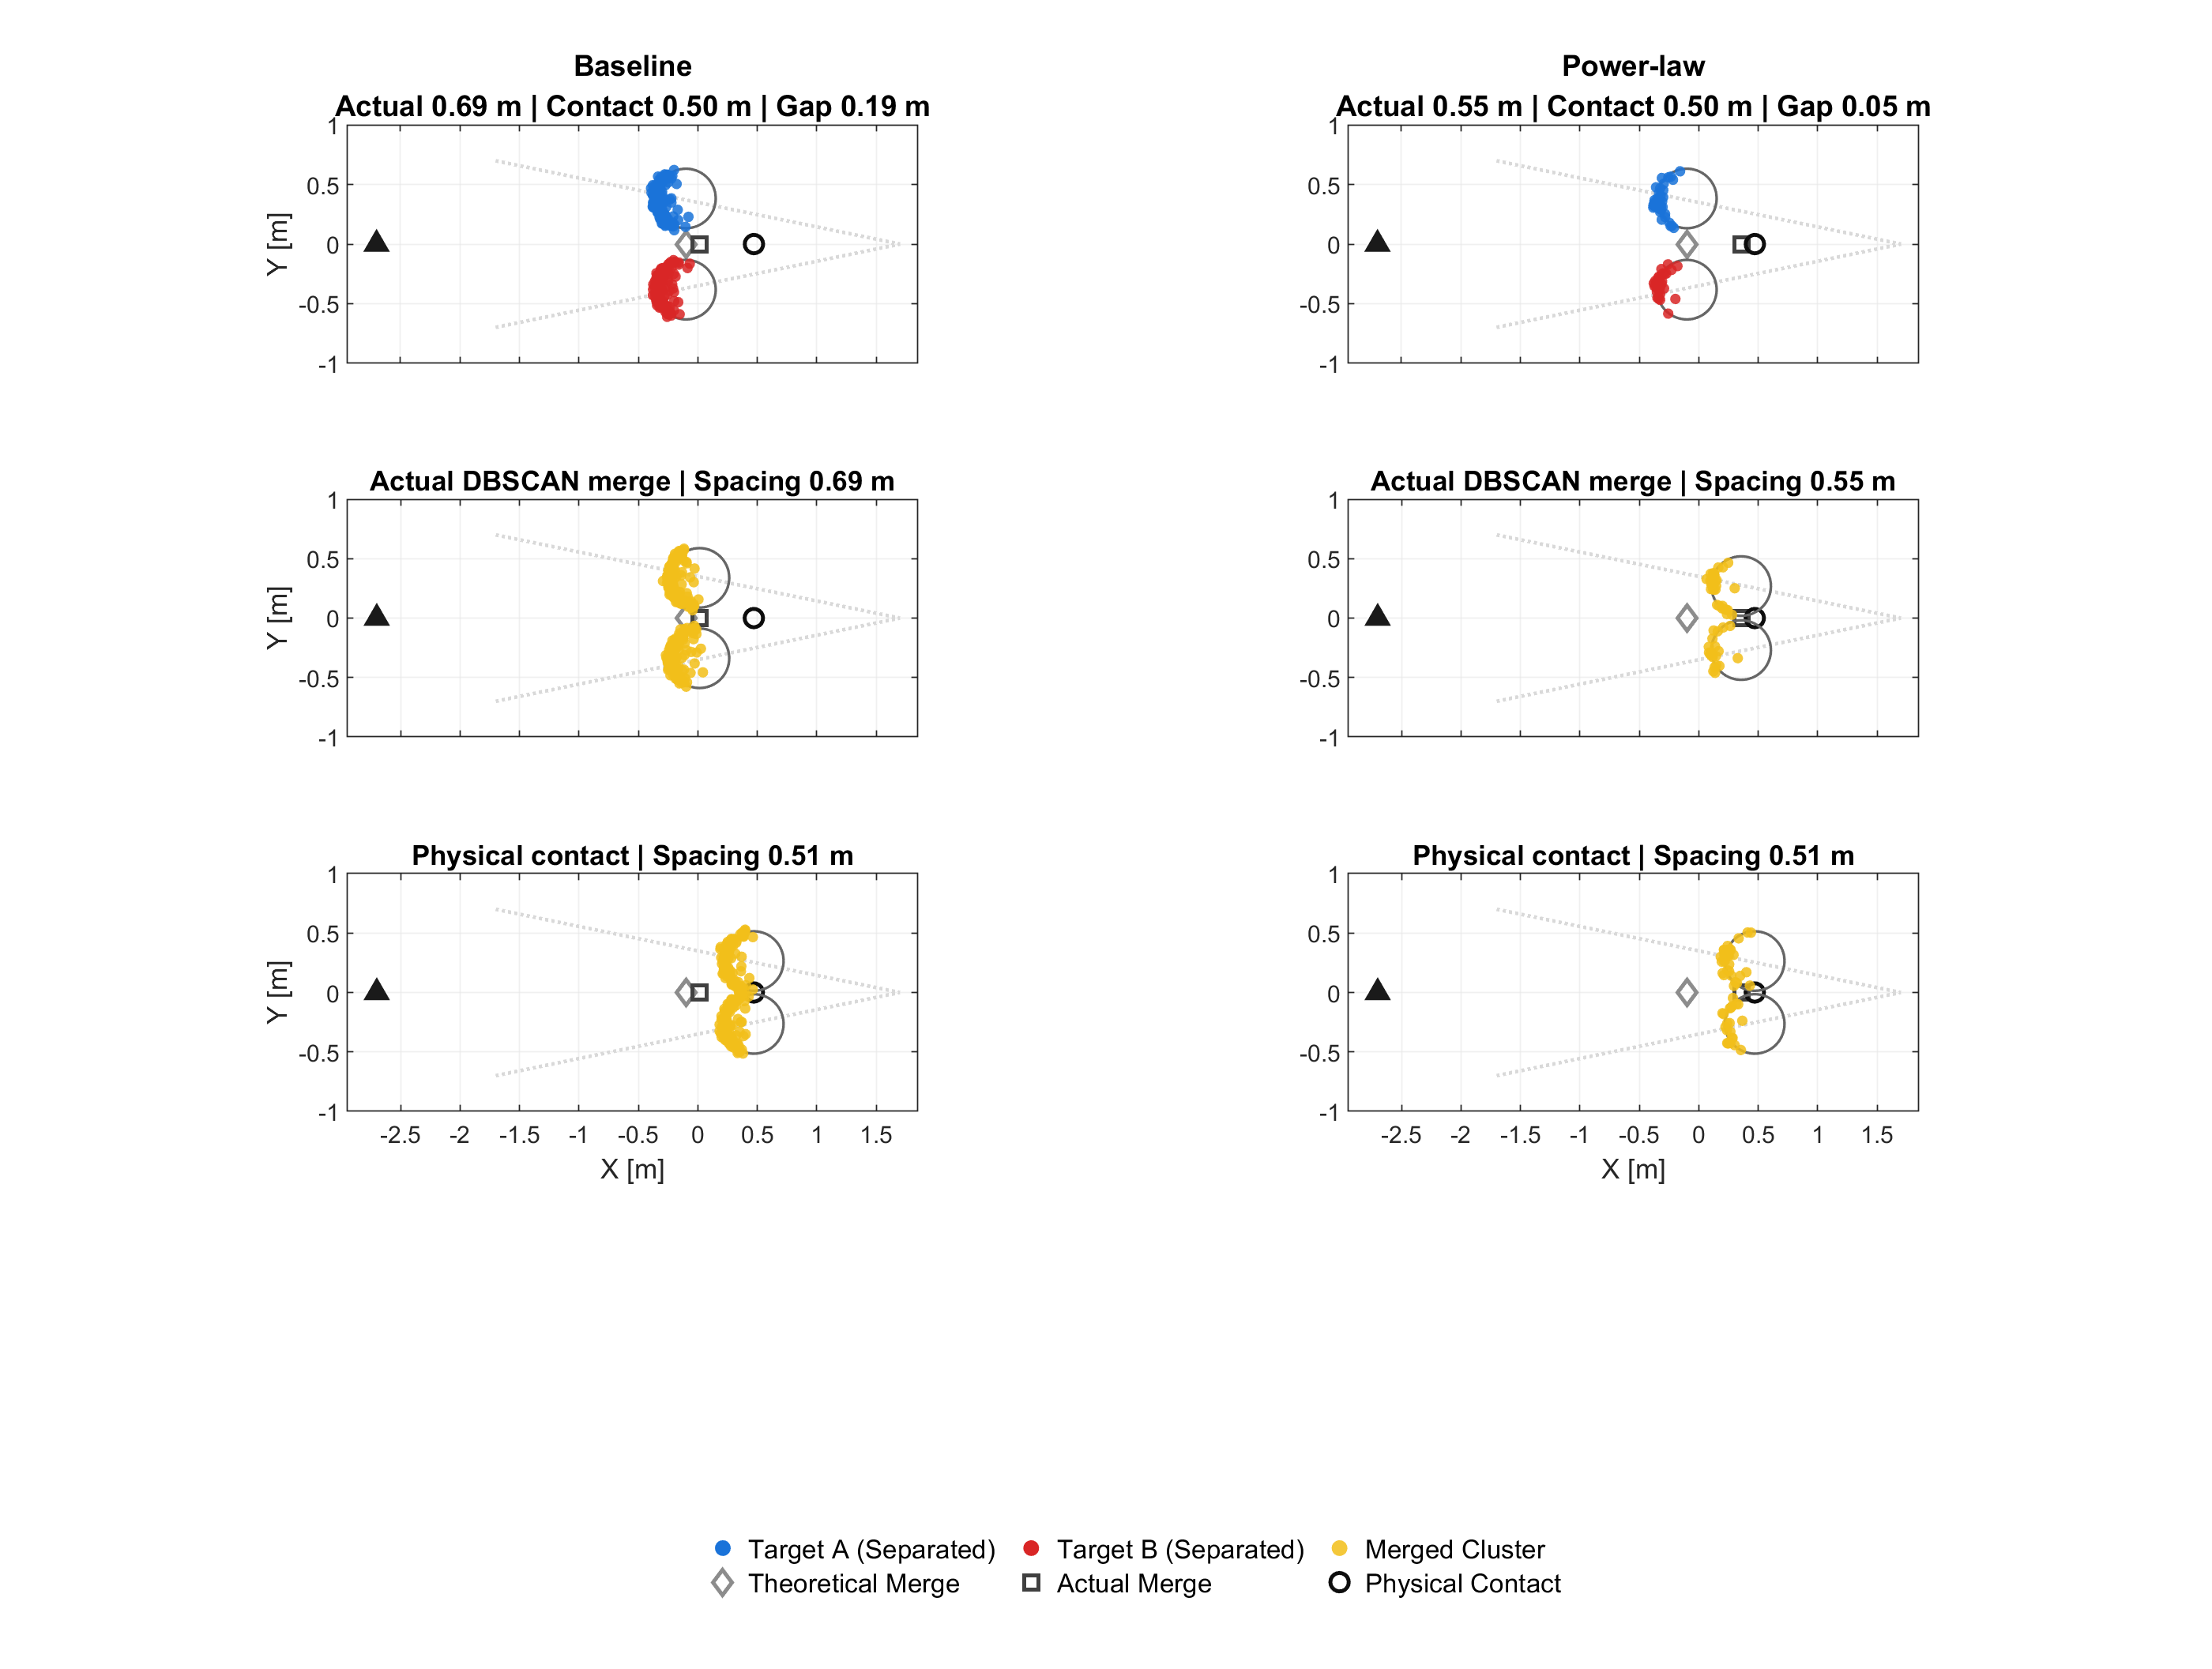
\includegraphics[width=0.95\linewidth]{Figure11.png}
    \captionof{figure}{Enlarged comparison of Baseline and Power-law bubble-buffer behavior.}
    \label{fig:aq6-baseline-powerlaw-detail}
\end{center}

Figure~\ref{fig:aq6-sigmoid-density-detail} gives the same enlarged comparison for the Sigmoid and Density models. The Sigmoid model merges at about $0.58~\mathrm{m}$, while the Density model merges at about $0.62~\mathrm{m}$. This makes the tradeoff more visible: all 3 active models reduce premature merging compared with the baseline, but they do not produce exactly the same point-cloud shape or merge spacing.

\begin{center}
    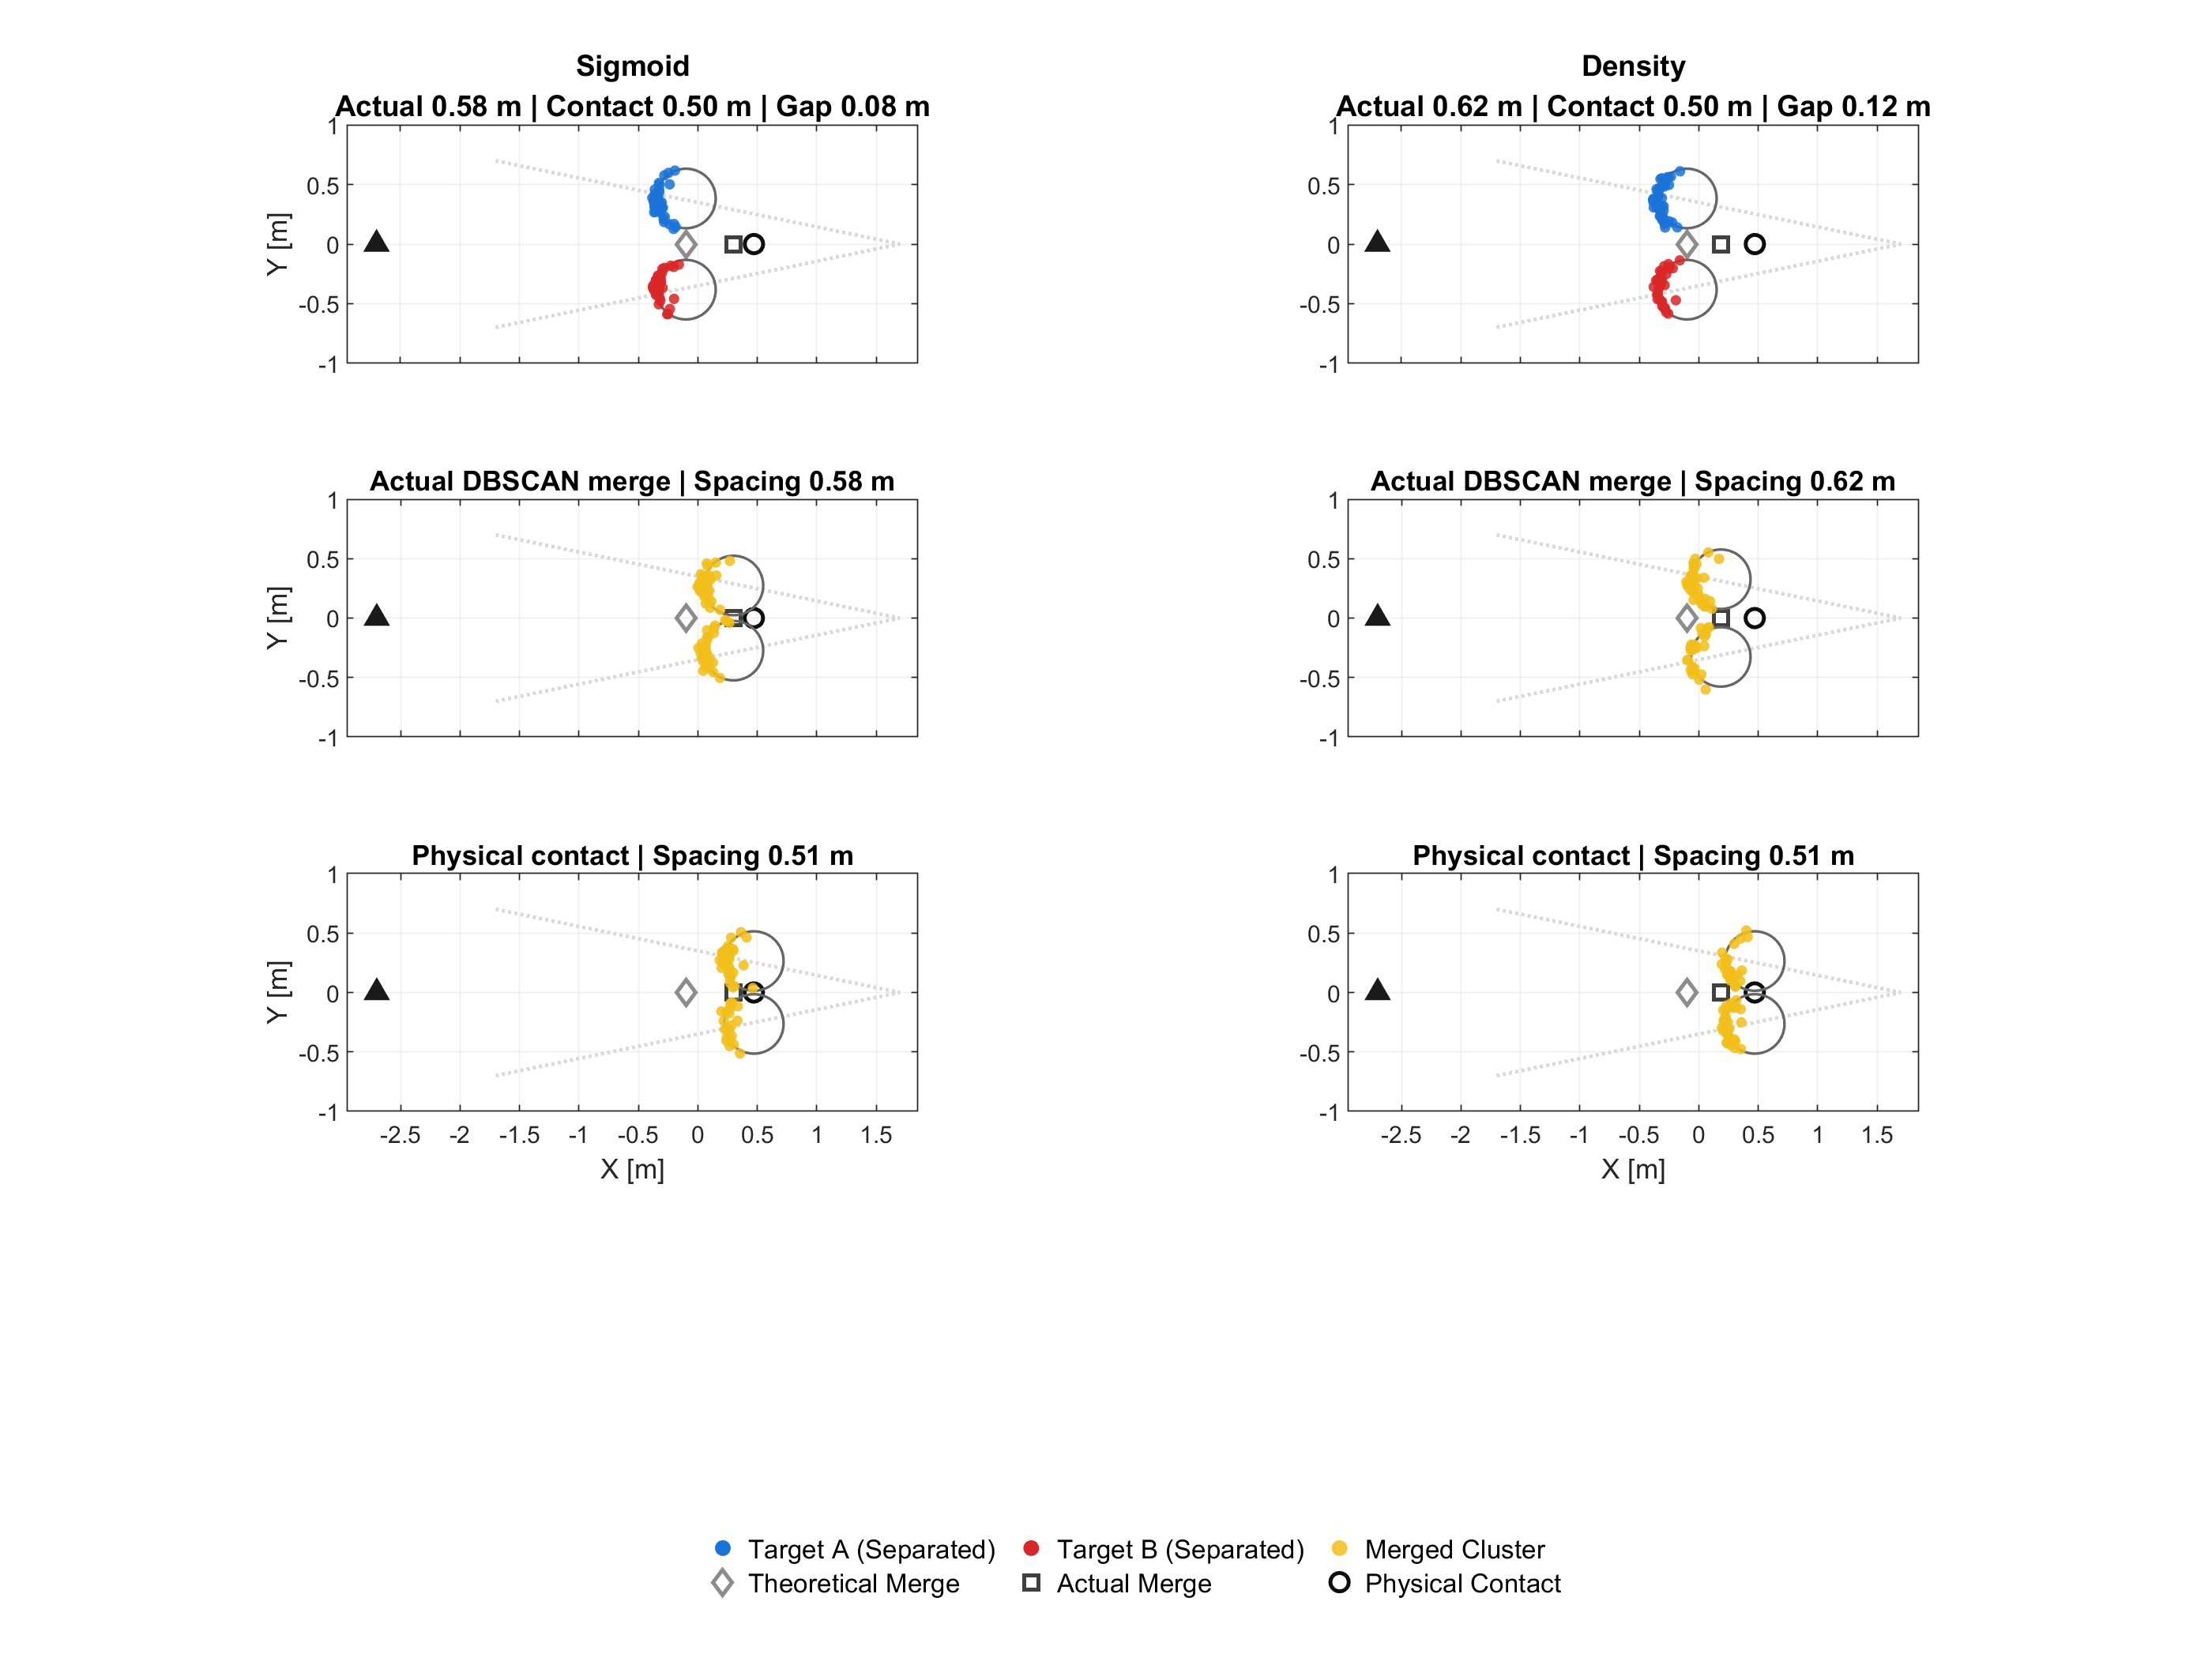
\includegraphics[width=0.95\linewidth]{Figure12.png}
    \captionof{figure}{Enlarged comparison of Sigmoid and Density bubble-buffer behavior.}
    \label{fig:aq6-sigmoid-density-detail}
\end{center}

Figure~\ref{fig:aq6-merge-zoom-detail} zooms into the actual DBSCAN merge frame for the 4 models. This view shows the boundary-point distribution in more detail. The active models keep fewer points near the facing boundary, so the connected cluster appears later and closer to physical contact.

\begin{center}
    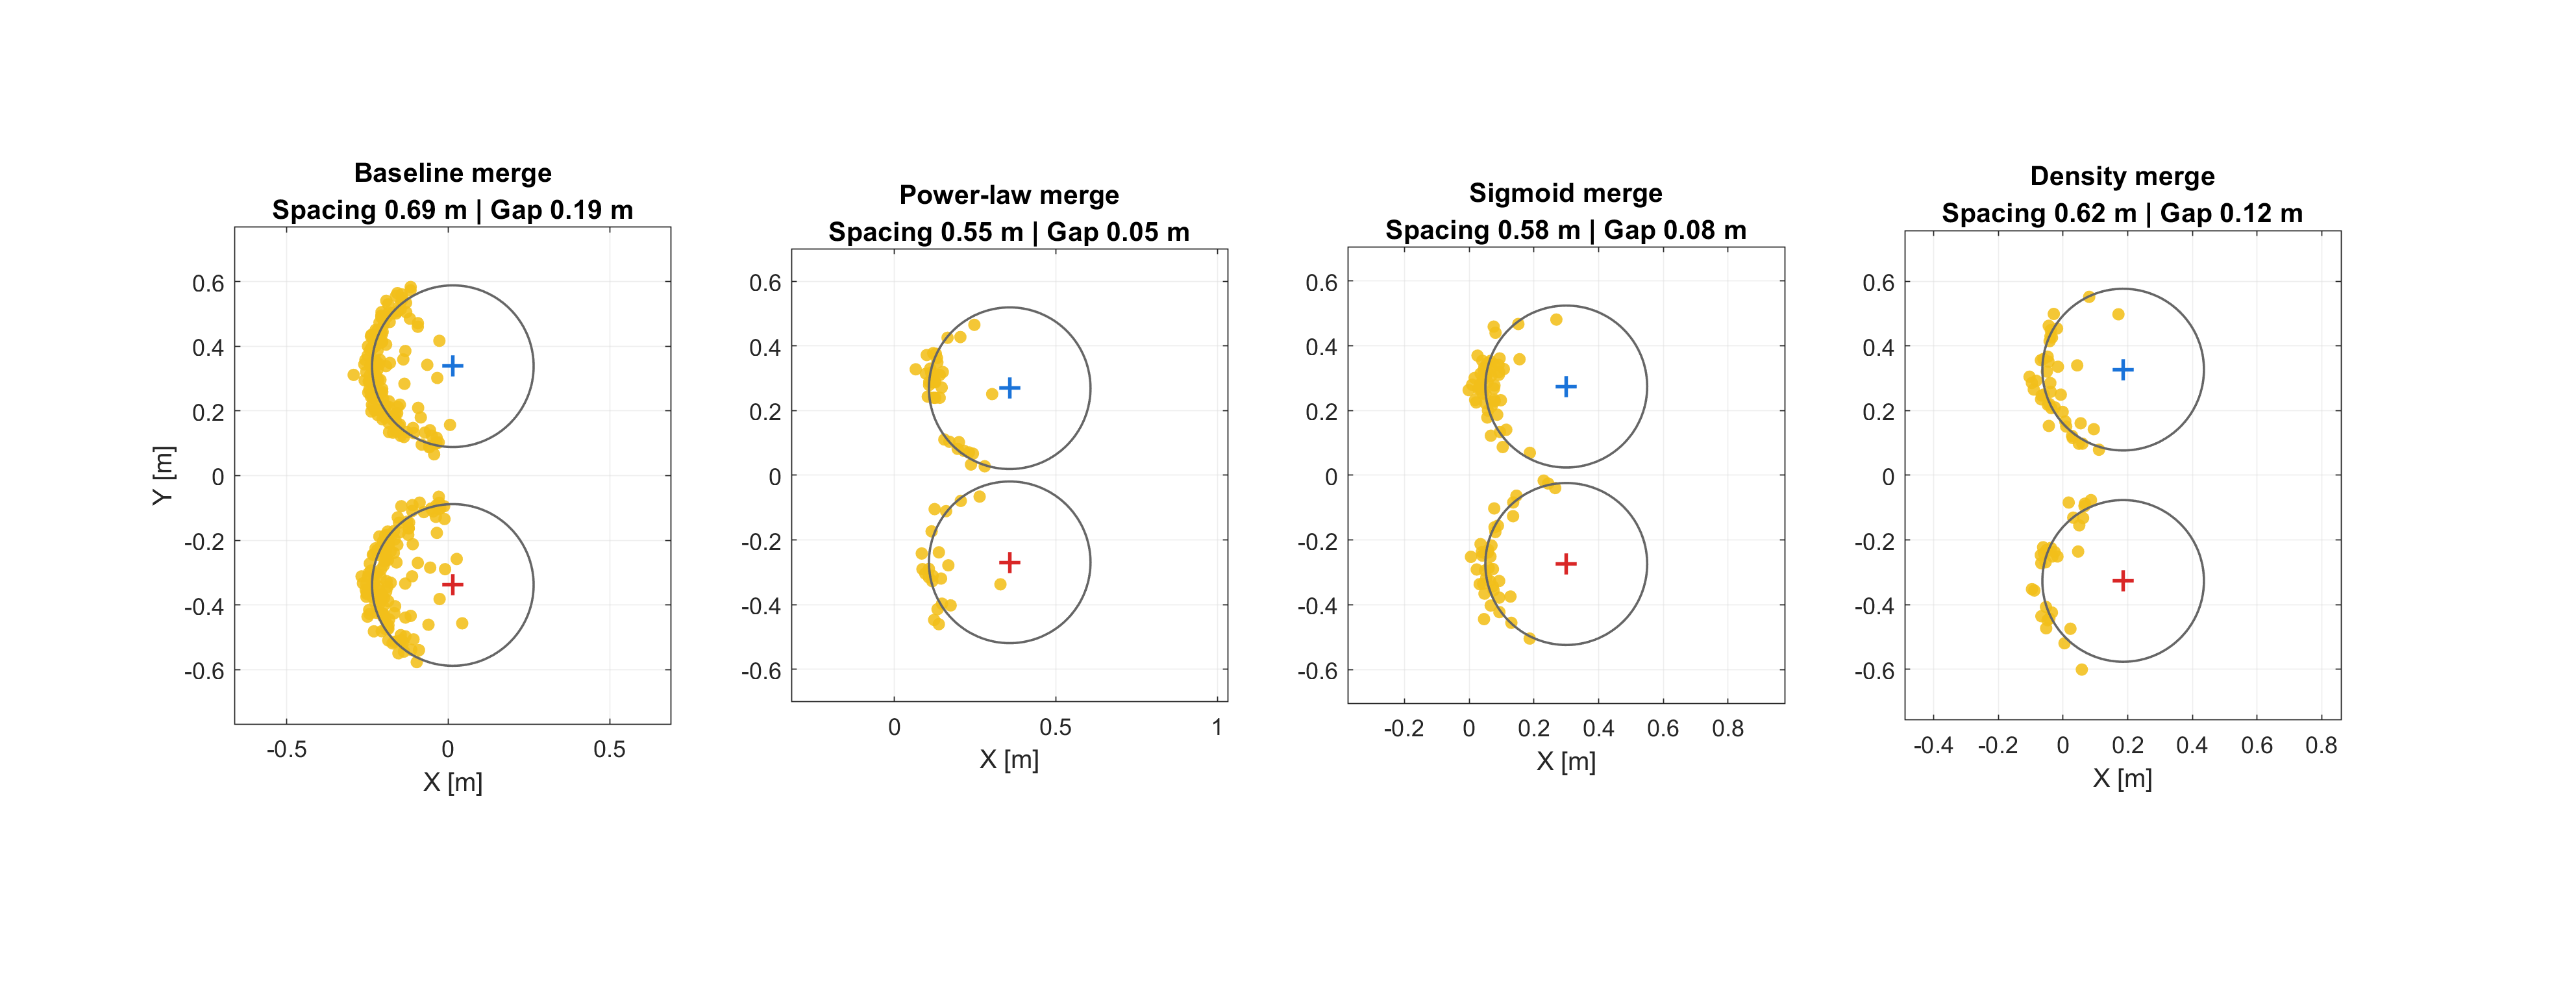
\includegraphics[width=0.95\linewidth]{Figure13.png}
    \captionof{figure}{Zoomed actual-merge views for Baseline, Power-law, Sigmoid, and Density models.}
    \label{fig:aq6-merge-zoom-detail}
\end{center}
\end{contentbox}
% ==========================================
\chapter{Literature Analysis}
% ==========================================
\begin{sectionintro}{Theoretical Models}
This appendix summarizes the main papers and the models that can be reused in the current project.
\end{sectionintro}

\boxitemtitle{Continuous Indoor Localization through LiDAR and IMU Sensor Fusion~\cite{xu2026indoorlocalization}}
\begin{contentbox}
    \textbf{KDRQ Model:} A KD-tree range query compares each incoming LiDAR point with a pre-built static background model. Points without nearby background neighbors are classified as foreground. \\
    \textbf{Application:} This is the baseline foreground segmentation strategy for ceiling-mounted LiDAR localization. It supports per-frame centroid extraction and provides a reference for evaluating single-person trajectory quality. \\
    \textbf{Additional Use:} The head-centroid idea can be extended to multi-person tracking by treating the head region as a more stable measurement source during partial body occlusion.
\end{contentbox}

\boxitemtitle{Person Tracking in Three-Dimensional Laser Range Data with Explicit Occlusion Adaption~\cite{schoeler2011occlusion}}
\begin{contentbox}
    \textbf{EOA Model:} The observation weight is adapted using ray-traced occlusion ratios. The expected number of observed points decreases when the visible ratio decreases. \\
    \textbf{Application:} This supports visible-ratio-based confidence modeling during partial and full occlusion. \\
    \textbf{Additional Use:} The same principle can be used to reduce the measurement weight in a Kalman or particle filter when a target is only partially visible.
\end{contentbox}

\boxitemtitle{Efficient Detection and Tracking of Human Using 3D LiDAR Sensor~\cite{gomez2023efficient}}
\begin{contentbox}
    \textbf{ROI-Tracking Model:} Predicted regions of interest are extracted before voxelization, segmentation, geometric classification, and tracking are applied only to high-probability target regions. \\
    \textbf{Application:} This justifies reducing computational cost by processing only dynamic or predicted regions, which supports real-time multi-person tracking. \\
    \textbf{Additional Use:} Its voting-style shape, normal, and shadow classifiers directly motivate the proposed Morphology and Visibility voters.
\end{contentbox}

\boxitemtitle{Multi-body Target Indoor Positioning System Based on Fusion of LiDAR and Monocular Camera~\cite{xiong2022multibody}}
\begin{contentbox}
    \textbf{MC Model:} Monocular-camera detections are mapped into the LiDAR point cloud using calibrated intrinsic and extrinsic parameters, so that human-related point clouds can be extracted more reliably. \\
    \textbf{Application:} This supports the idea that additional sensing information can resolve ambiguities when pure point-cloud clustering becomes unreliable. \\
    \textbf{Additional Use:} Although this internship focuses on LiDAR-only tracking, the camera-fusion result can serve as an upper-bound comparison for multi-target separability.
\end{contentbox}

\boxitemtitle{Dynablox: Real-Time Detection of Diverse Dynamic Objects in Complex Environments~\cite{schmid2023dynablox}}
\begin{contentbox}
    \textbf{Dynablox Model:} Dynamic objects are detected when points appear in previously high-confidence free space. A volumetric map is maintained to distinguish static structure from newly occupied regions. \\
    \textbf{Application:} This justifies free-space-based dynamic object detection and introduces evaluation metrics such as dynamic-point IoU, real-time FPS, and robustness under complex indoor geometry. \\
    \textbf{Additional Use:} High-confidence free-space reasoning can be adapted to identify unexpected target reappearance after occlusion.
\end{contentbox}

\boxitemtitle{Deep Learning-Based Real-Time Human Detection System Using LiDAR Data for Smart Healthcare Monitoring~\cite{kalashtari2024deeplidar}}
\begin{contentbox}
    \textbf{DL Model:} 3D LiDAR data are converted into 2D reflectivity images and processed with a YOLO-based detector for real-time human detection. \\
    \textbf{Application:} This provides a learning-based comparison method and shows that reflectivity images can support human detection. \\
    \textbf{Additional Use:} The reflectivity-image idea can inspire a lightweight non-DL descriptor for distinguishing human clothing from robot surfaces.
\end{contentbox}

\boxitemtitle{Roadside LiDAR Vehicle Detection and Tracking Using Range and Intensity Background Subtraction~\cite{zhang2022roadside}}
\begin{contentbox}
    \textbf{RIBS Model:} Range and intensity channels are transformed into structured spatio-temporal matrices. Background and foreground are separated using DMD and CFTA. \\
    \textbf{Application:} This supports the use of non-geometric LiDAR channels, especially range and intensity, for background subtraction and dynamic target extraction. \\
    \textbf{Additional Use:} The structured matrix representation can inspire a time-window view of ceiling-LiDAR point density and reflectivity changes.
\end{contentbox}

\boxitemtitle{Advancing Multi-Object Tracking through Occlusion-Awareness and Trajectory Optimization~\cite{advancingMOT2024}}
\begin{contentbox}
    \textbf{Layered Association Model:} Occluded targets are separated into priority layers for sequential data association. Track states such as Wait, Restore, and Delete are used to handle uncertain observations. \\
    \textbf{Application:} This supports the Wait/Recover state logic in the proposed 3-Voter Mechanism. \\
    \textbf{Additional Use:} The layered idea can be combined with depth ordering so that near targets are processed before far targets in multi-person occlusion reasoning.
\end{contentbox}

\boxitemtitle{Occlusion-Aware Multi-Object Tracking via Expected Probability of Detection~\cite{epodMOT2024}}
\begin{contentbox}
    \textbf{EPoD Model:} Detection probability is adjusted according to expected visibility under object occlusion. Lower visibility leads to lower measurement confidence. \\
    \textbf{Application:} This supports visible-ratio-based measurement weighting in Kalman or Gaussian-mixture tracking. \\
    \textbf{Additional Use:} EPoD can be used as a formal bridge between geometric shadow modeling and probabilistic track confidence.
\end{contentbox}

\boxitemtitle{Reflectivity-Aware LiDAR-Inertial Odometry and Mapping~\cite{dong2023rliom}}
\begin{contentbox}
    \textbf{Reflectivity-Aware Model:} Reflectivity is used as an additional LiDAR attribute to improve residual computation, local mapping, pseudo-visual image generation, and loop detection. \\
    \textbf{Application:} This supports exploiting non-geometric LiDAR information, such as reflectivity or intensity, to improve point selection, map consistency, and trajectory reliability. \\
    \textbf{Additional Use:} Reflectivity can become a target fingerprint for mixed human-robot tracking, especially when geometry alone is ambiguous during cluster merging.
\end{contentbox}

\newpage
% ==========================================
\chapter{Weekly Reports}
% ==========================================
\begin{sectionintro}{Overview}
This appendix provides a chronological record of progress and supervisor discussions. It highlights technical milestones and future plans.
\end{sectionintro}

\boxitemtitle{Week 1: Orientation}
\begin{contentbox}
    \begin{itemize}[leftmargin=*, nosep]
        \item Attended Yiyun Xu's thesis defense to understand the research background of indoor localization.
        \item Analyzed the core methodology of the previous work, focusing on LiDAR-IMU sensor fusion, KDRQ, and head-centroid extraction.
        \item Identified the key research challenges related to dynamic target tracking and occlusion in cluttered indoor environments.
    \end{itemize}
\end{contentbox}

\boxitemtitle{Week 2: Occlusion Geometry}
\begin{contentbox}
    \begin{itemize}[leftmargin=*, nosep]
        \item Derived the geometric occlusion model and quantified the blind-zone length as $e = \frac{h \cdot d}{H-h}$.
        \item Evaluated L-shaped point-cloud data to analyze the geometric characteristics of human targets during movement.
    \end{itemize}
\end{contentbox}

\boxitemtitle{Week 3: Literature Review}
\begin{contentbox}
    \begin{itemize}[leftmargin=*, nosep]
        \item Reviewed 3 papers related to occlusion-aware tracking.
        \item Extracted relevant ideas for observation weighting, visibility reasoning, and multi-target association.
    \end{itemize}
\end{contentbox}

\boxitemtitle{Week 4: Model Upgrade}
\begin{contentbox}
    \begin{itemize}[leftmargin=*, nosep]
        \item Created the project log file on Overleaf.
        \item Extended the blind-zone model from 1D length to a 2D fan-shaped shadow, forming the basis of the occlusion testing model.
        \item Proposed several simulation scenarios for multi-target tracking and merging analysis.
    \end{itemize}
\end{contentbox}

\boxitemtitle{Week 5: Simulation Framework and Occlusion Modeling}
\begin{contentbox}
    \begin{itemize}[leftmargin=*, nosep]
        \item Built a 3-module framework: scenario-driven point-cloud generation, core multi-target tracking, and performance evaluation.
        \item Improved simulation realism by including target geometry, target number, motion patterns, point noise, 1-sided sparsity, gait-induced centroid oscillation, occlusion shadows, and cluster merging.
        \item Analyzed the merging problem between 2 moving targets and identified a sparsity-induced separation margin that can delay premature DBSCAN merging.
        \item Extended the occlusion discussion from 2-target cases to more complex multi-target cases, including X-crossing motion and potential ID loss.
    \end{itemize}
\end{contentbox}

\boxitemtitle{Week 6: Distance Attenuation and Sensor-Resolution Discussion}
\begin{contentbox}
    \begin{itemize}[leftmargin=*, nosep]
        \item Introduced a point-count attenuation factor to describe the decrease in point-cloud density as the target-LiDAR distance increases.
        \item Extracted the attenuation factor from Xu's data and fitted a regression model after excluding unreliable boundary points.
        \item Connected the attenuation model with the Ouster angular-resolution limitation: when the target is farther away, fewer laser rays hit the object.
        \item Discussed with supervisors that another researcher may have a method for compensating accuracy degradation caused by distance and angular resolution.
        \item Summarized the potential of using additional LiDAR information beyond geometry, especially reflectivity, to improve robustness under sparse or degraded point-cloud conditions.
        \item Received the R-LIOM paper and planned to study how reflectivity can support the current tracking model.
    \end{itemize}
\end{contentbox}

\boxitemtitle{Week 7: Wrap-Up and Reporting}
\begin{contentbox}
    \begin{itemize}[leftmargin=*, nosep]
        \item Wrapped up the final research report.
        \item Reviewed the R-LIOM paper and summarized its relevance to reflectivity-aware tracking.
        \item Drafted the 3-Voter Mechanism and the causal chain of multi-target degradation.
    \end{itemize}
\end{contentbox}

\boxitemtitle{Week 8: Preparation for defense}
\begin{contentbox}
    \begin{itemize}[leftmargin=*, nosep]
        \item Arranging files and prepare for a defense presentation at June 16th
        \item Orientation for thesis project
    \end{itemize}
\end{contentbox}

\newpage
\newpage
\addcontentsline{toc}{chapter}{References}
\bibliographystyle{IEEEtran}
\bibliography{references}

\end{document}
